\documentclass[11pt,letterpaper]{article}
\input{headings}
\usepackage{soul}

\newcommand \recipeName {Asian Zucchini}
\newcommand \fileName {AsianZucchini}

\chead{\recipeName}

\begin{document}
\input{title}

Zucchini is a great Summer squash, however cooking it can be tricky. I have found out that the secret is to pretty much not cook it at all, similar to the technique used in Chinese stir frying. However, it is difficult to impart flavour into the squash with such a brief cooking time. The techniques that I introduce into this recipe aim to impart flavour into this Summer squash without cooking it for long. The idea is remove the seeds and then to salt it ahead and thus remove some of the water, and then to impart flavour to the oil before introducing the squash to it. Asian

\begin{description}

\item[Ingredients:]\ \\
	\begin{itemize}
	\item 1 large zucchini or two small ones
	\item 1 clove of garlic
	\item 3 or 4 small hot peppers
	\item 1 tablespoon of chopped chives (or parsley)
	\item 1 1/2 tablespoons of cooking olive
	\item 1/8 teaspoon of salt
        \item 1 tablespoon of soy sauce
        \item 1 1/2 tablespoon of ginger
        \item 1/2 lime
        \item 1/2 tablespoon of sesame oil
	\end{itemize}

\item[Procedure:]\ \\
	\begin{enumerate}
	\item {\bf Prepare the Zucchini}
	\begin{itemize}
	\item Cut the zucchini lenghtwise in half and then cut each half lenghwise in half.
	\item With a small knife, cut the seeds out of the zucchini. Discard the seeds.
	\item Cut the zucchini into a small dice (about 1 cm cube pieces).
	\item  Put the diced zucchini in a bowl and sprinkle with the with the salt and soy sauce.
	\item Let stand for at least 20 minutes.
	\end{itemize}
	\item {\bf Flavour the oil}
	\begin{itemize}
        \item Place a fine mash strainer over a small bowl to have it ready.
	\item Slice the garlic, the hot pepper, and the ginger.
	\item Put the oil in a frying pan and put the garlic, ginger and hot pepper in the cold oil.
	\item Cook over moderate heat until the oil warms up through and you can smell the garlic and ginger.
	\item Using a heat-proof spatula drain the oil over the strainer and reserve until ready to cook.
	\end{itemize}
	\item{\bf Drain and sautee the zucchini}
	\begin{itemize}
	\item Put the zucchini on a strainer to drain and discard the water.
	\item Heat the flavoured oil over moderate heat until very hot, but not smoking.
	\item Add the zucchini to the hot oil, and the chives if using, and stir fry for about 90 seconds. You should just warm the zucchini through but for it to still be crisp.
        \item Add the sesame oil
	\item Remove to a plate, sprinkle with the lime juice and serve immediately.	
        \item Serve over young spinach leaves or with arugula.
	\end{itemize}
	\end{enumerate}
\end{description}
\begin{table}
\begin{tabular}{cccc}
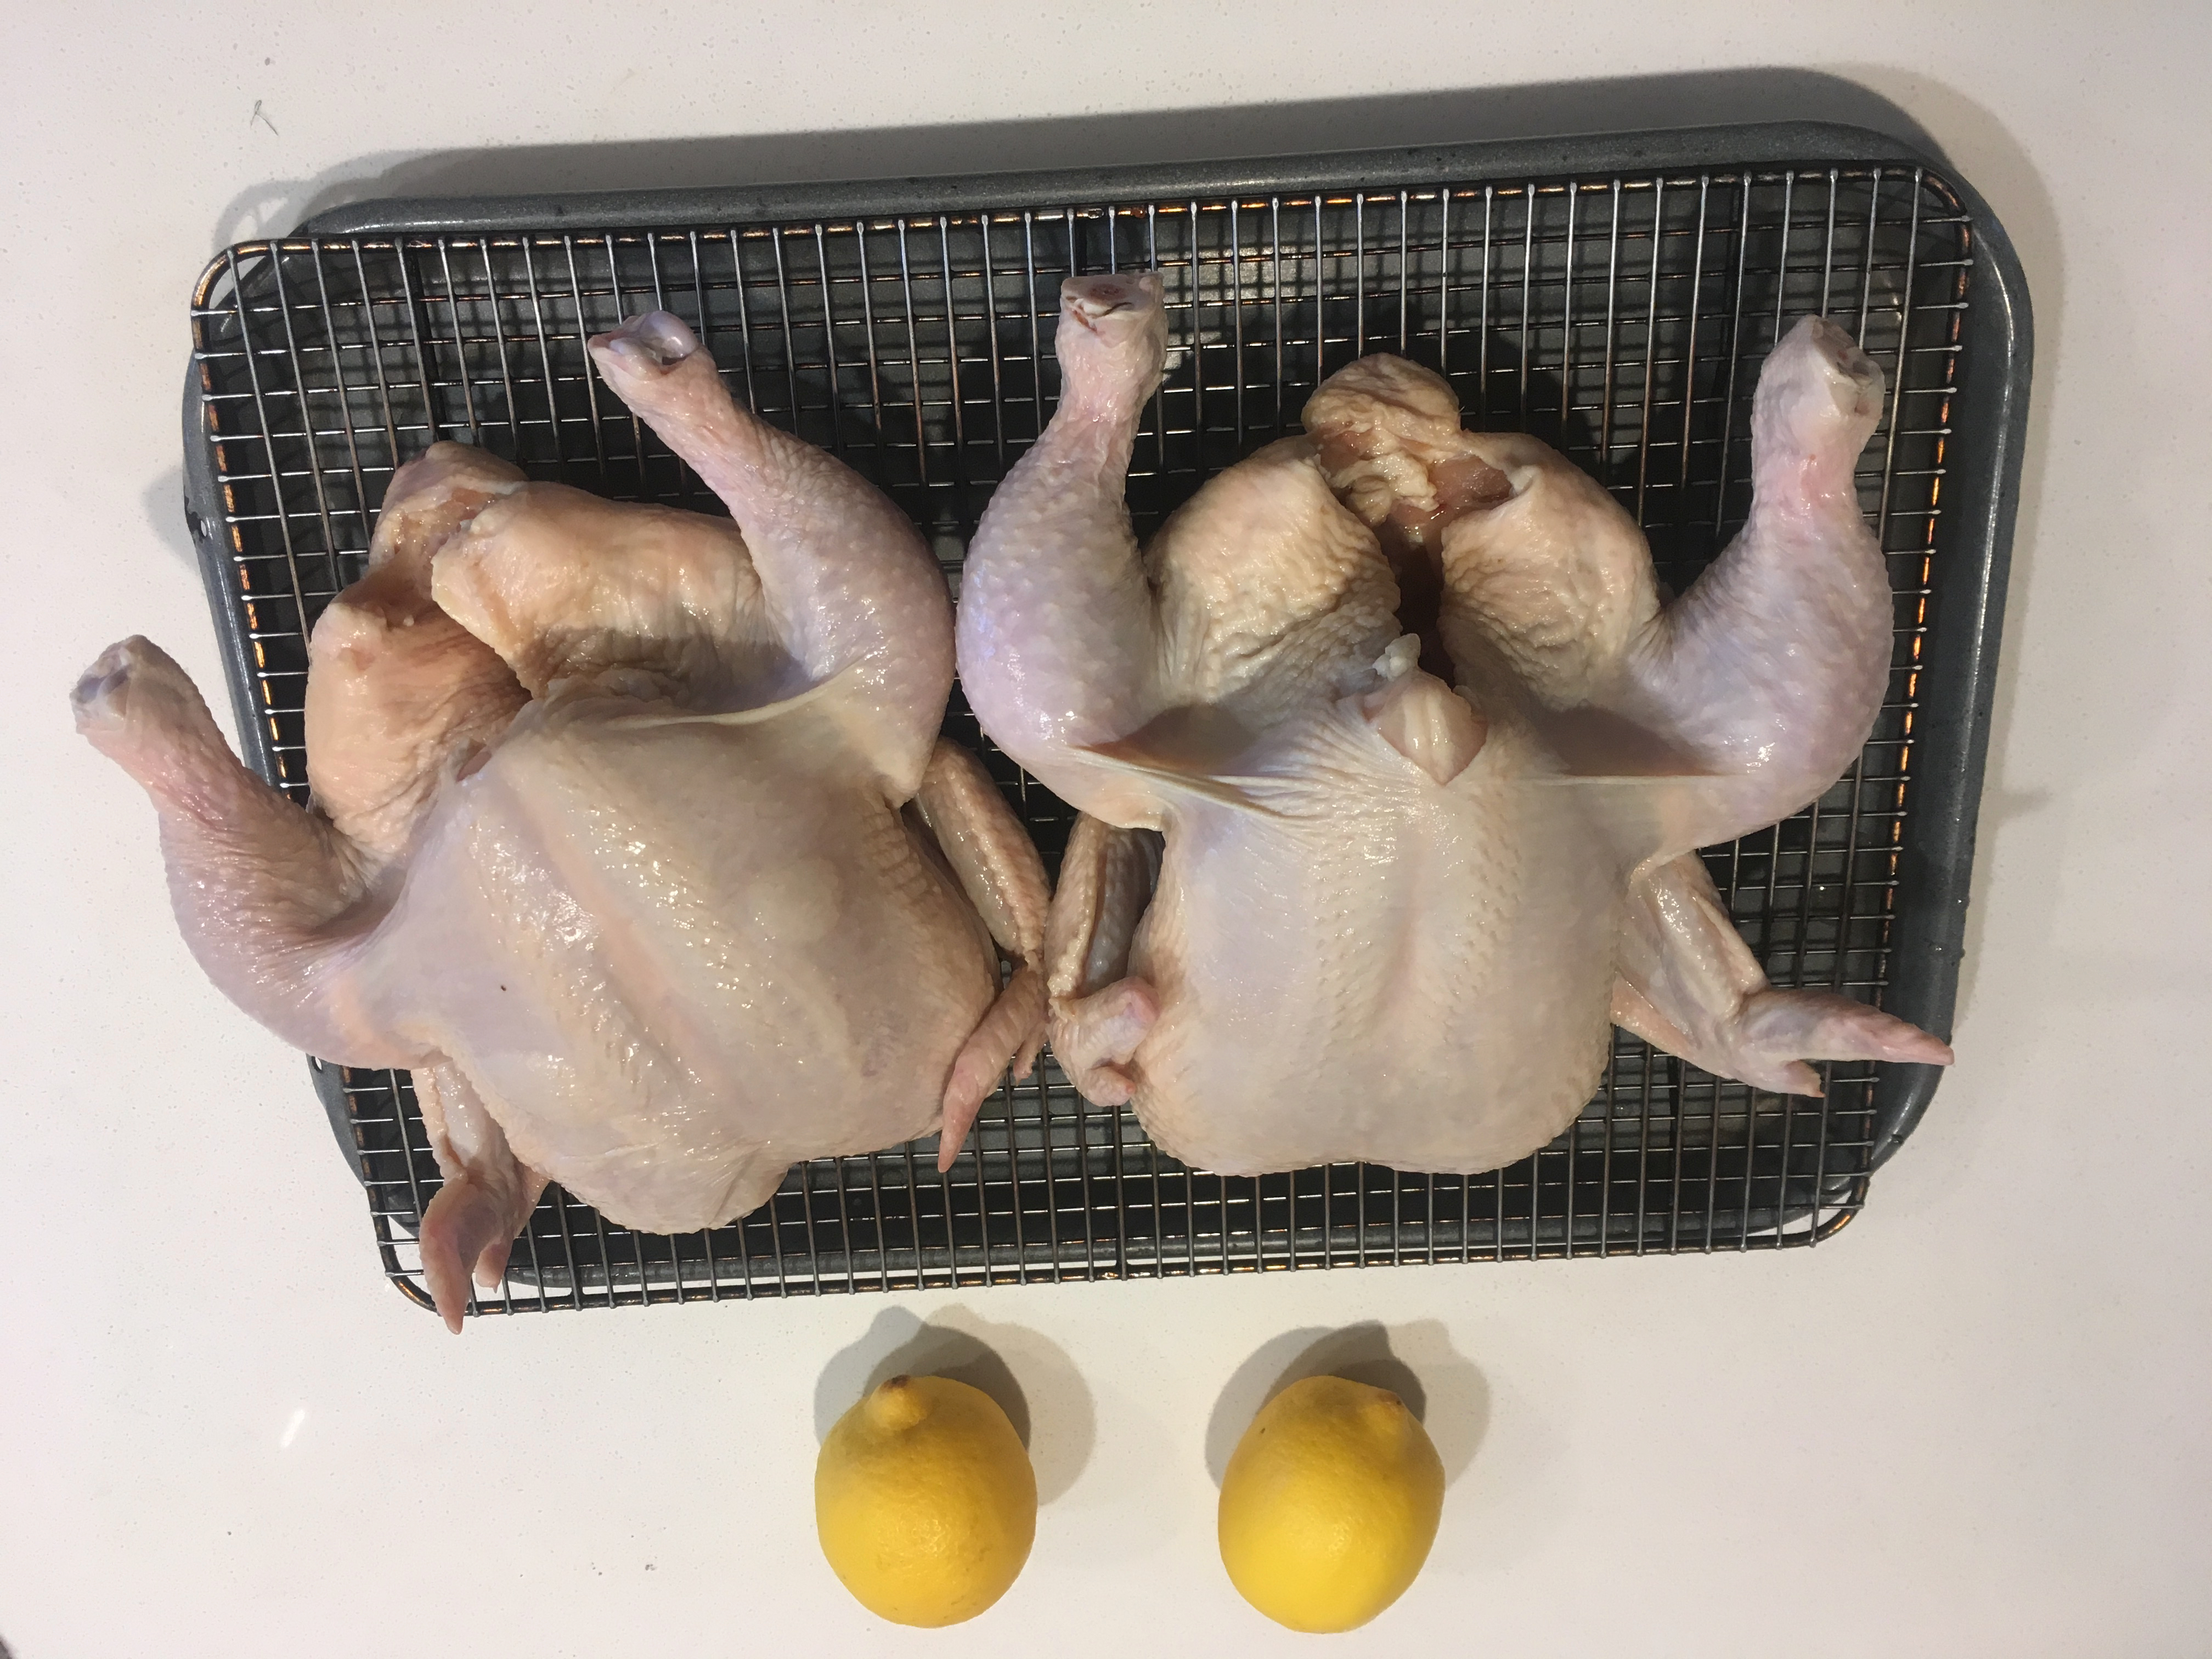
\includegraphics[width=0.25\textwidth]{\imageDir/\fileName/IMG_3197.jpg} &
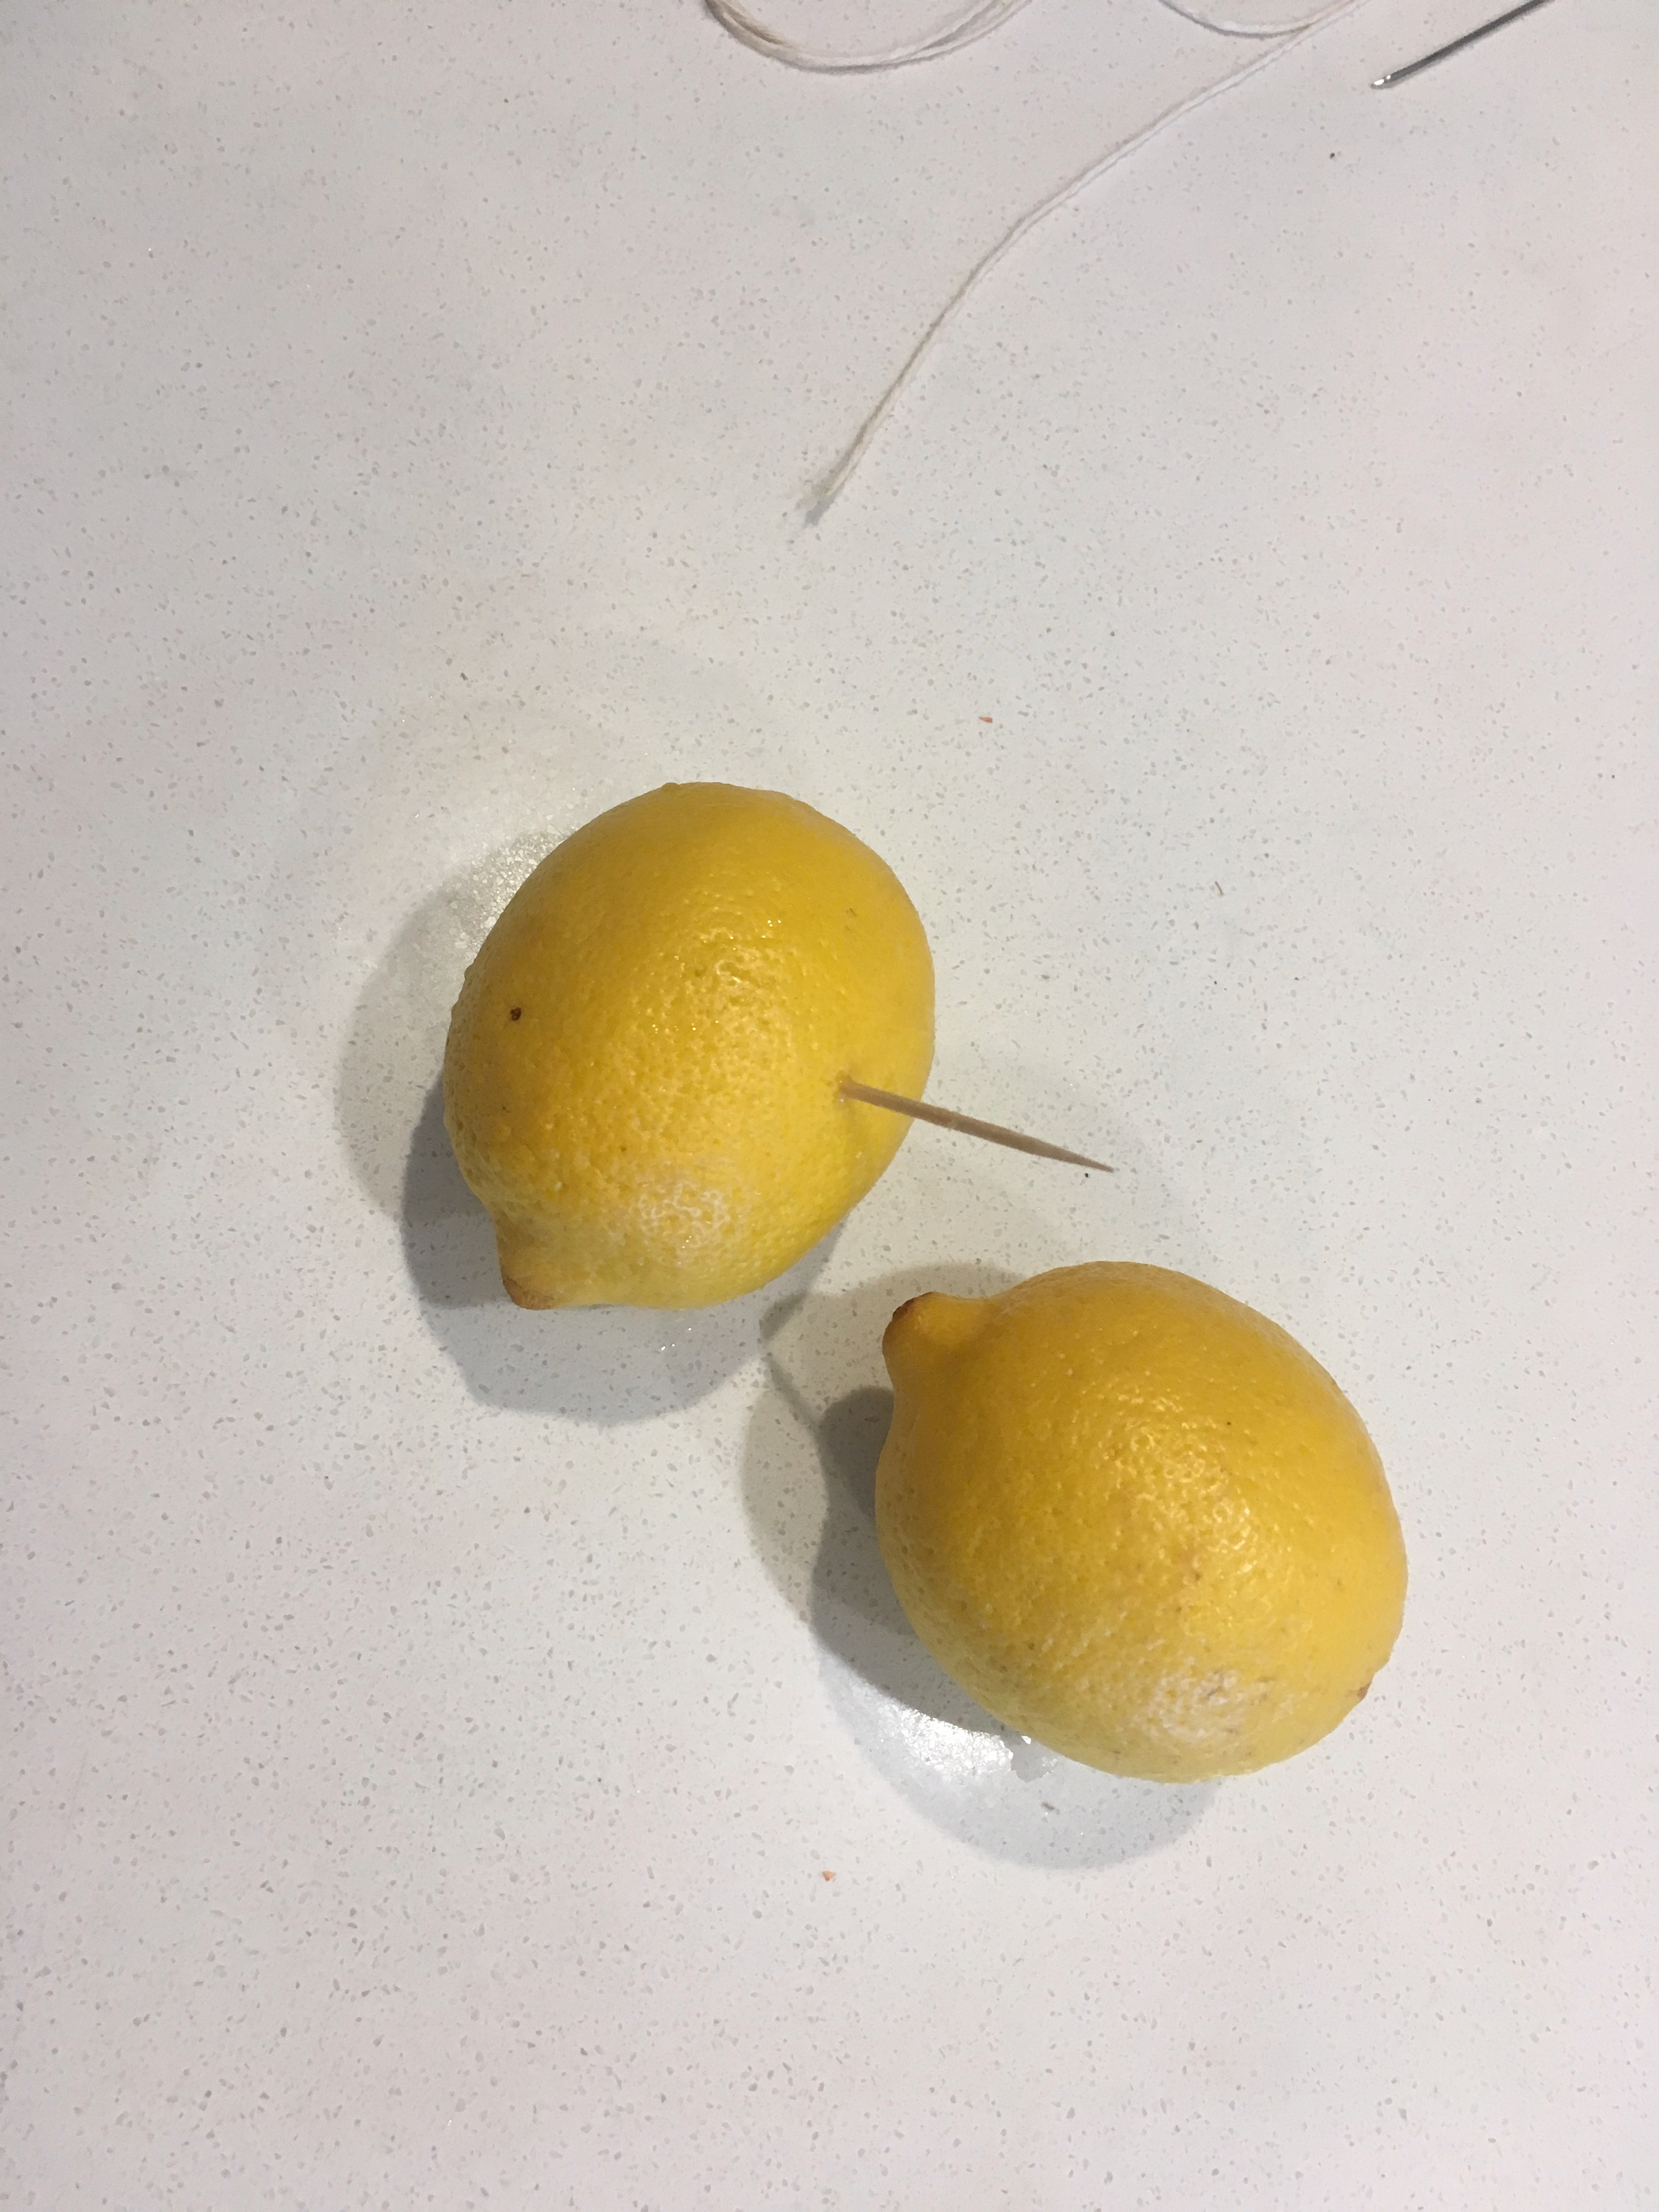
\includegraphics[width=0.25\textwidth]{\imageDir/\fileName/IMG_3212.jpg} &
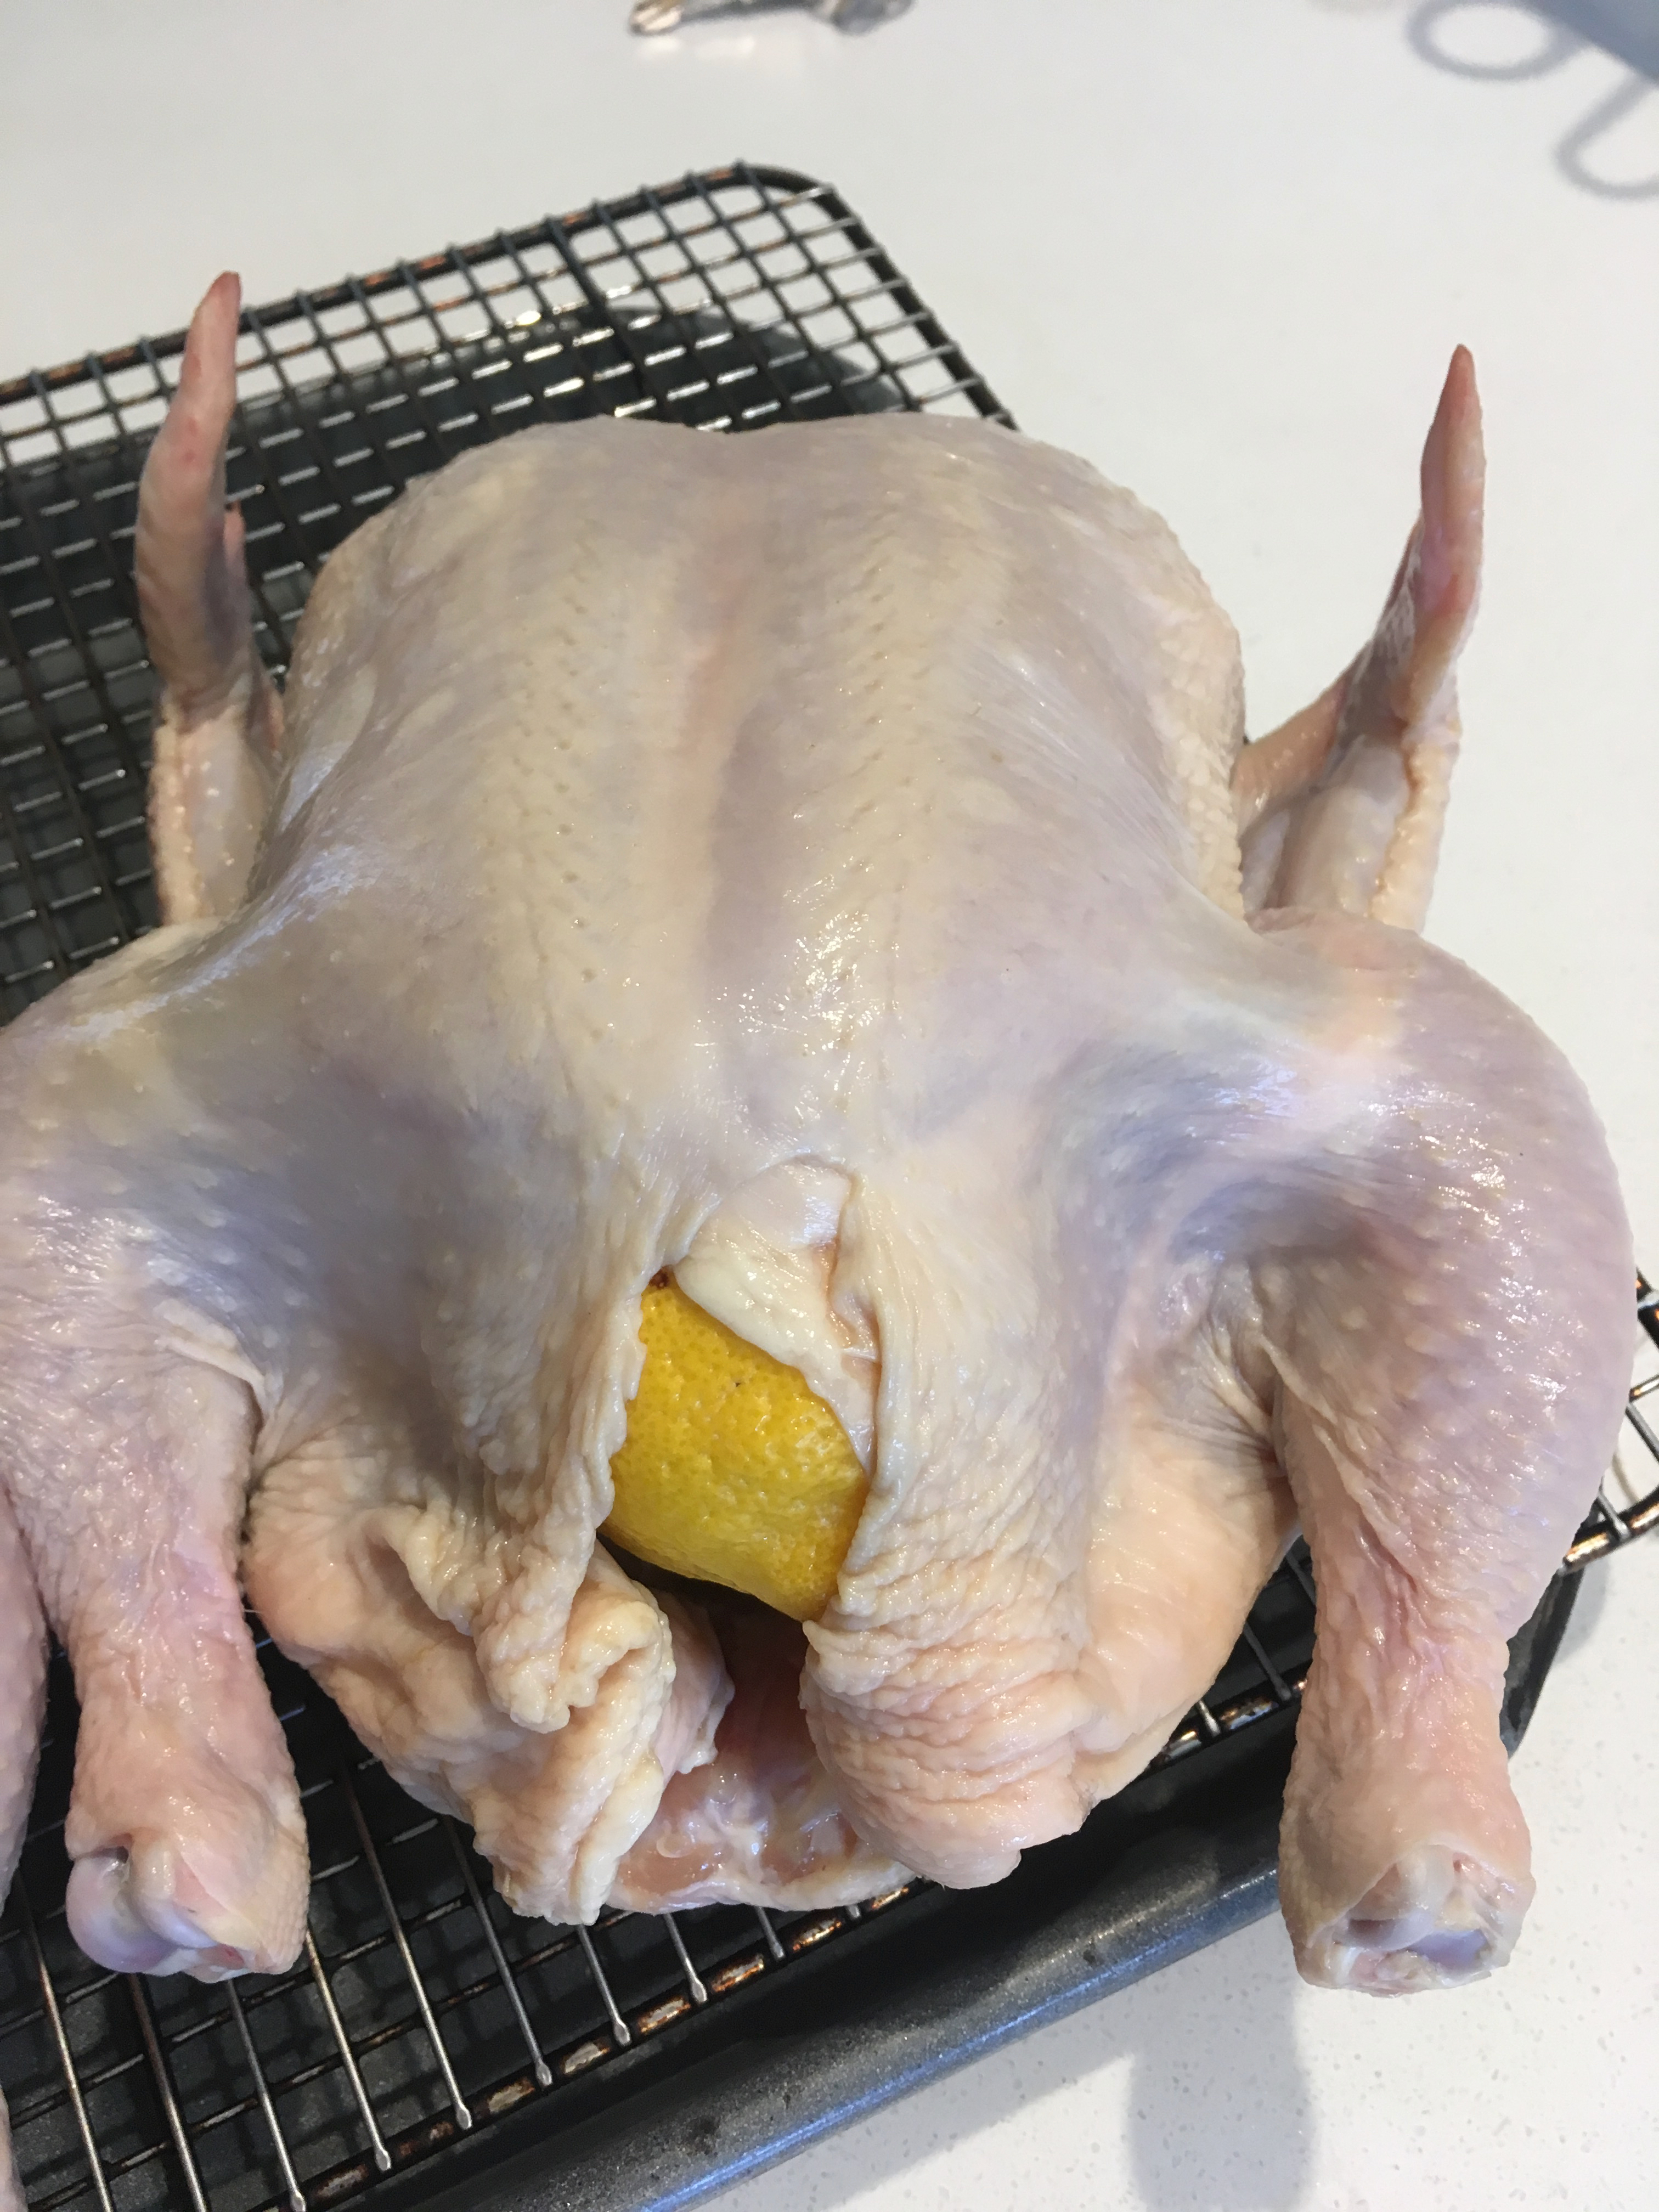
\includegraphics[width=0.25\textwidth]{\imageDir/\fileName/IMG_3213.jpg} \\

\includegraphics[width=0.25\textwidth]{\imageDir/\fileName/IMG_3206.jpg} &
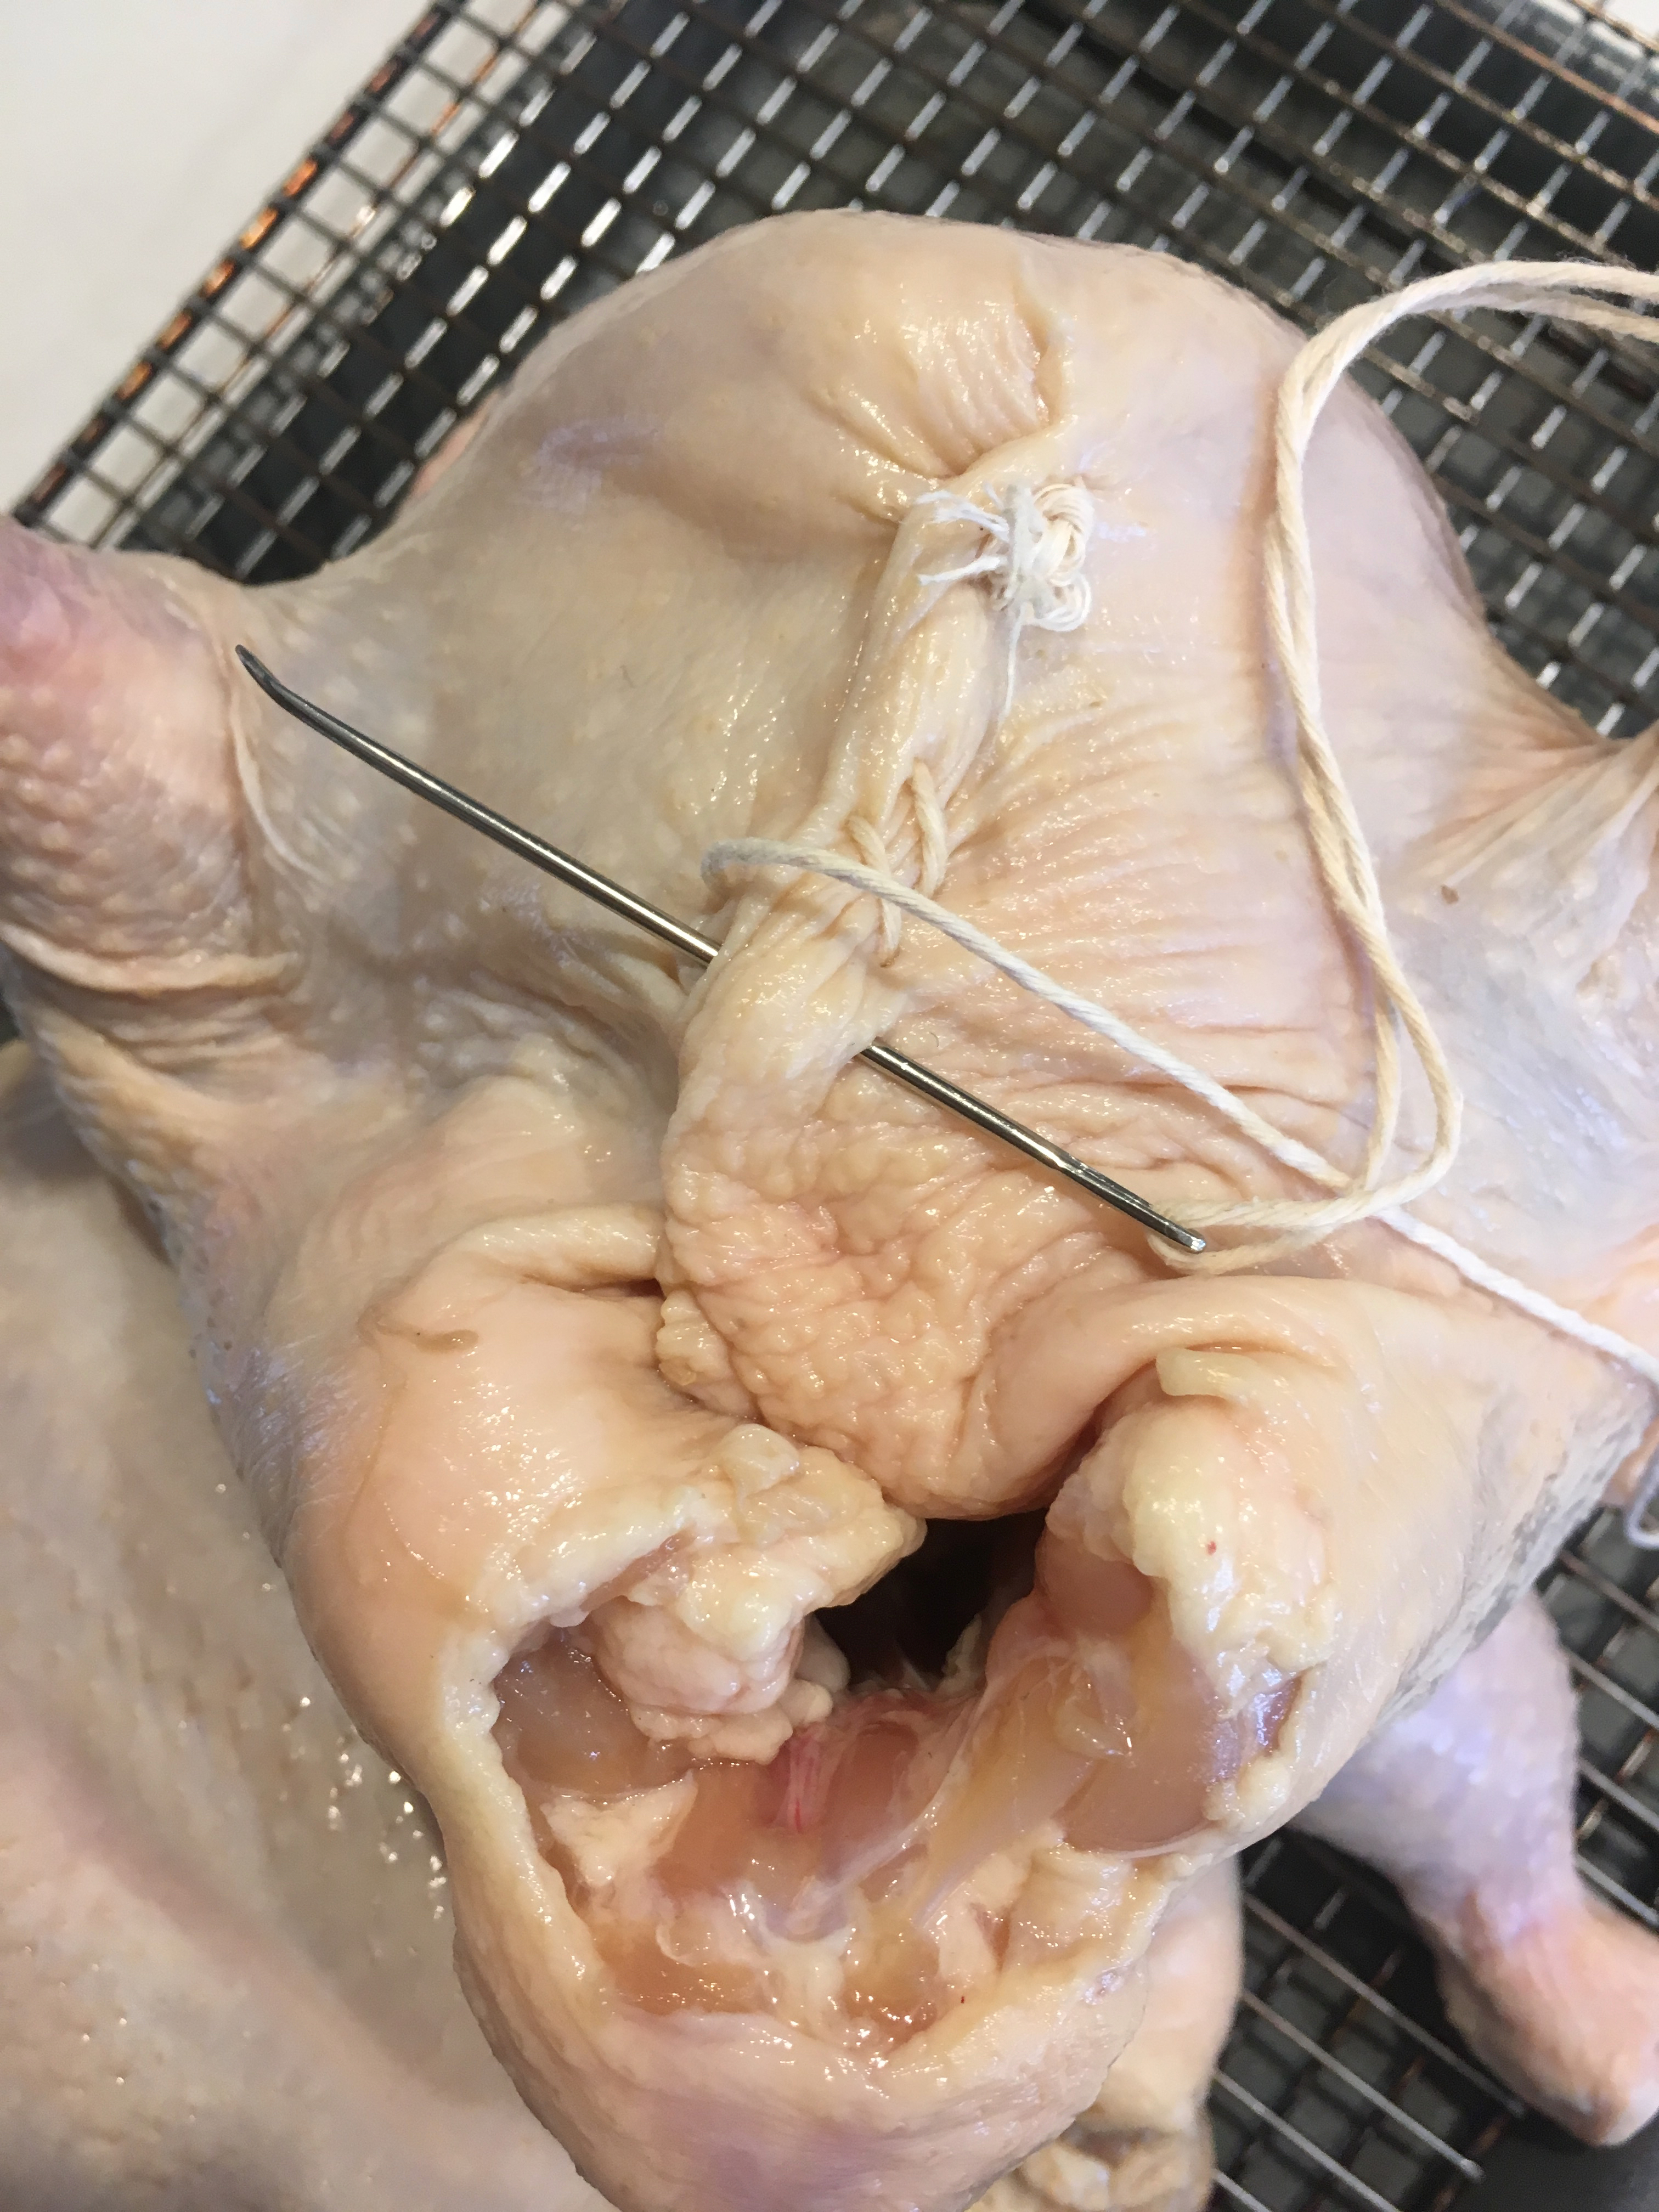
\includegraphics[width=0.25\textwidth]{\imageDir/\fileName/IMG_3214.jpg} &
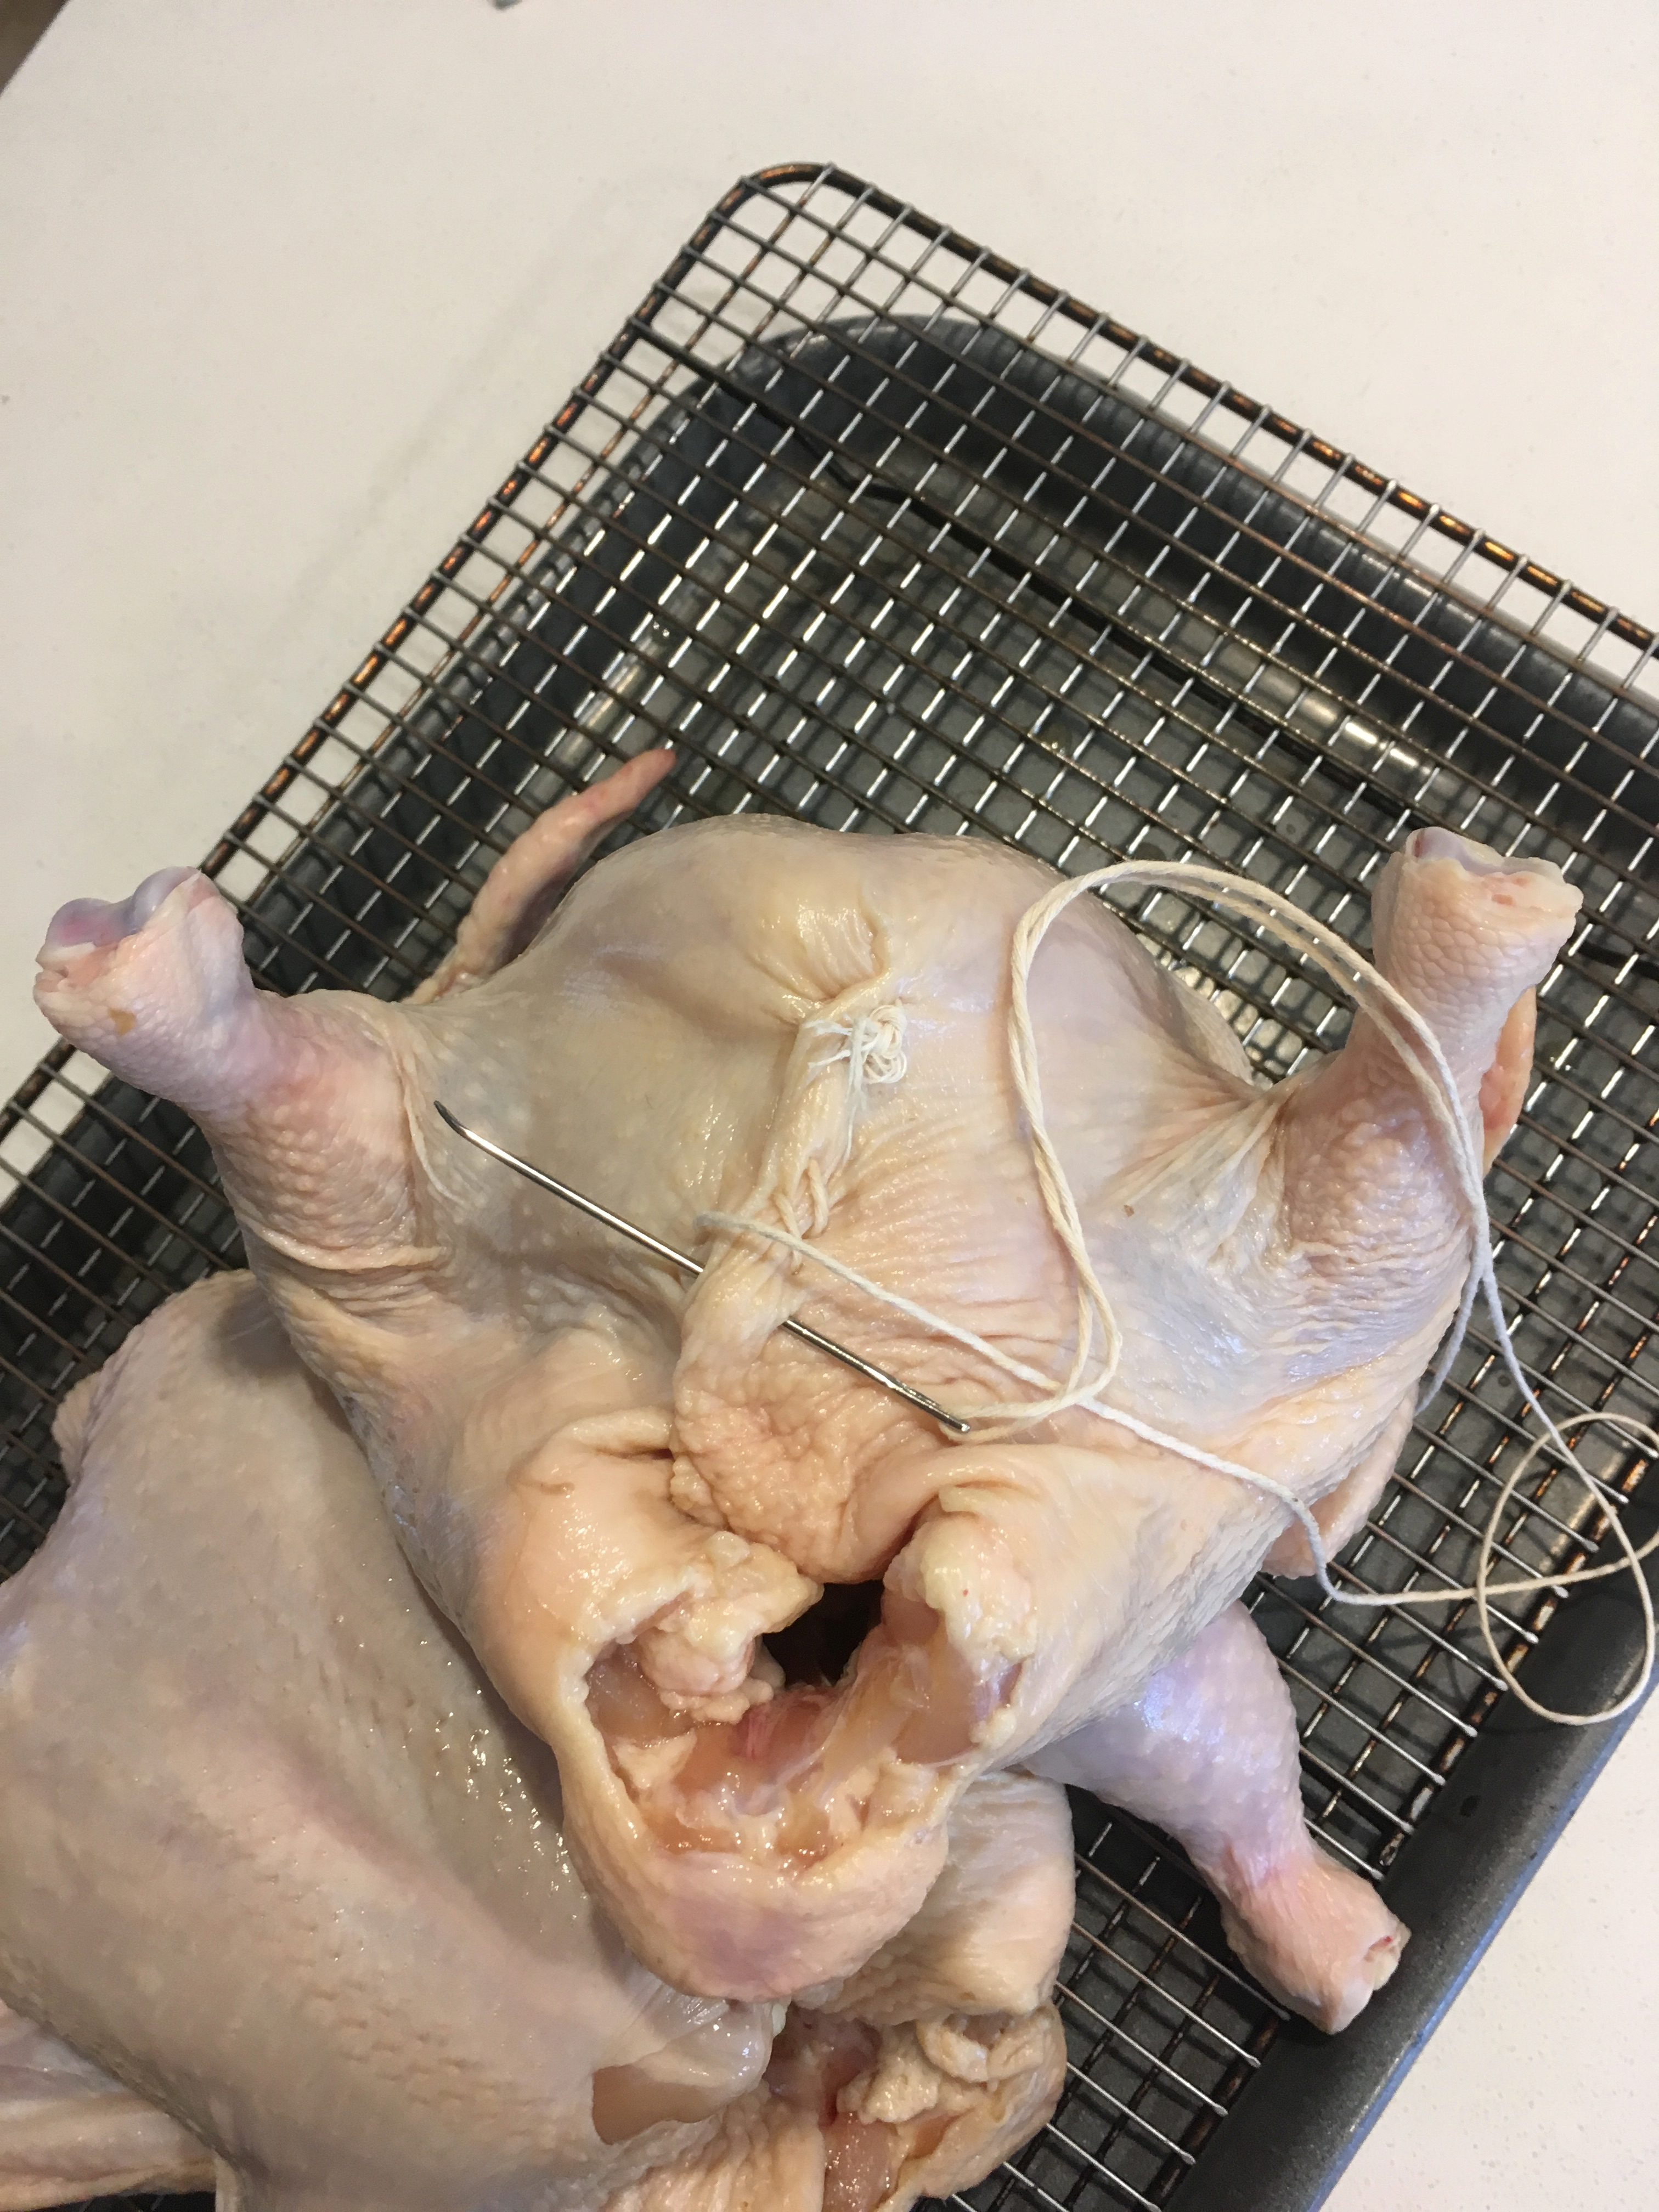
\includegraphics[width=0.25\textwidth]{\imageDir/\fileName/IMG_3216.jpg} \\
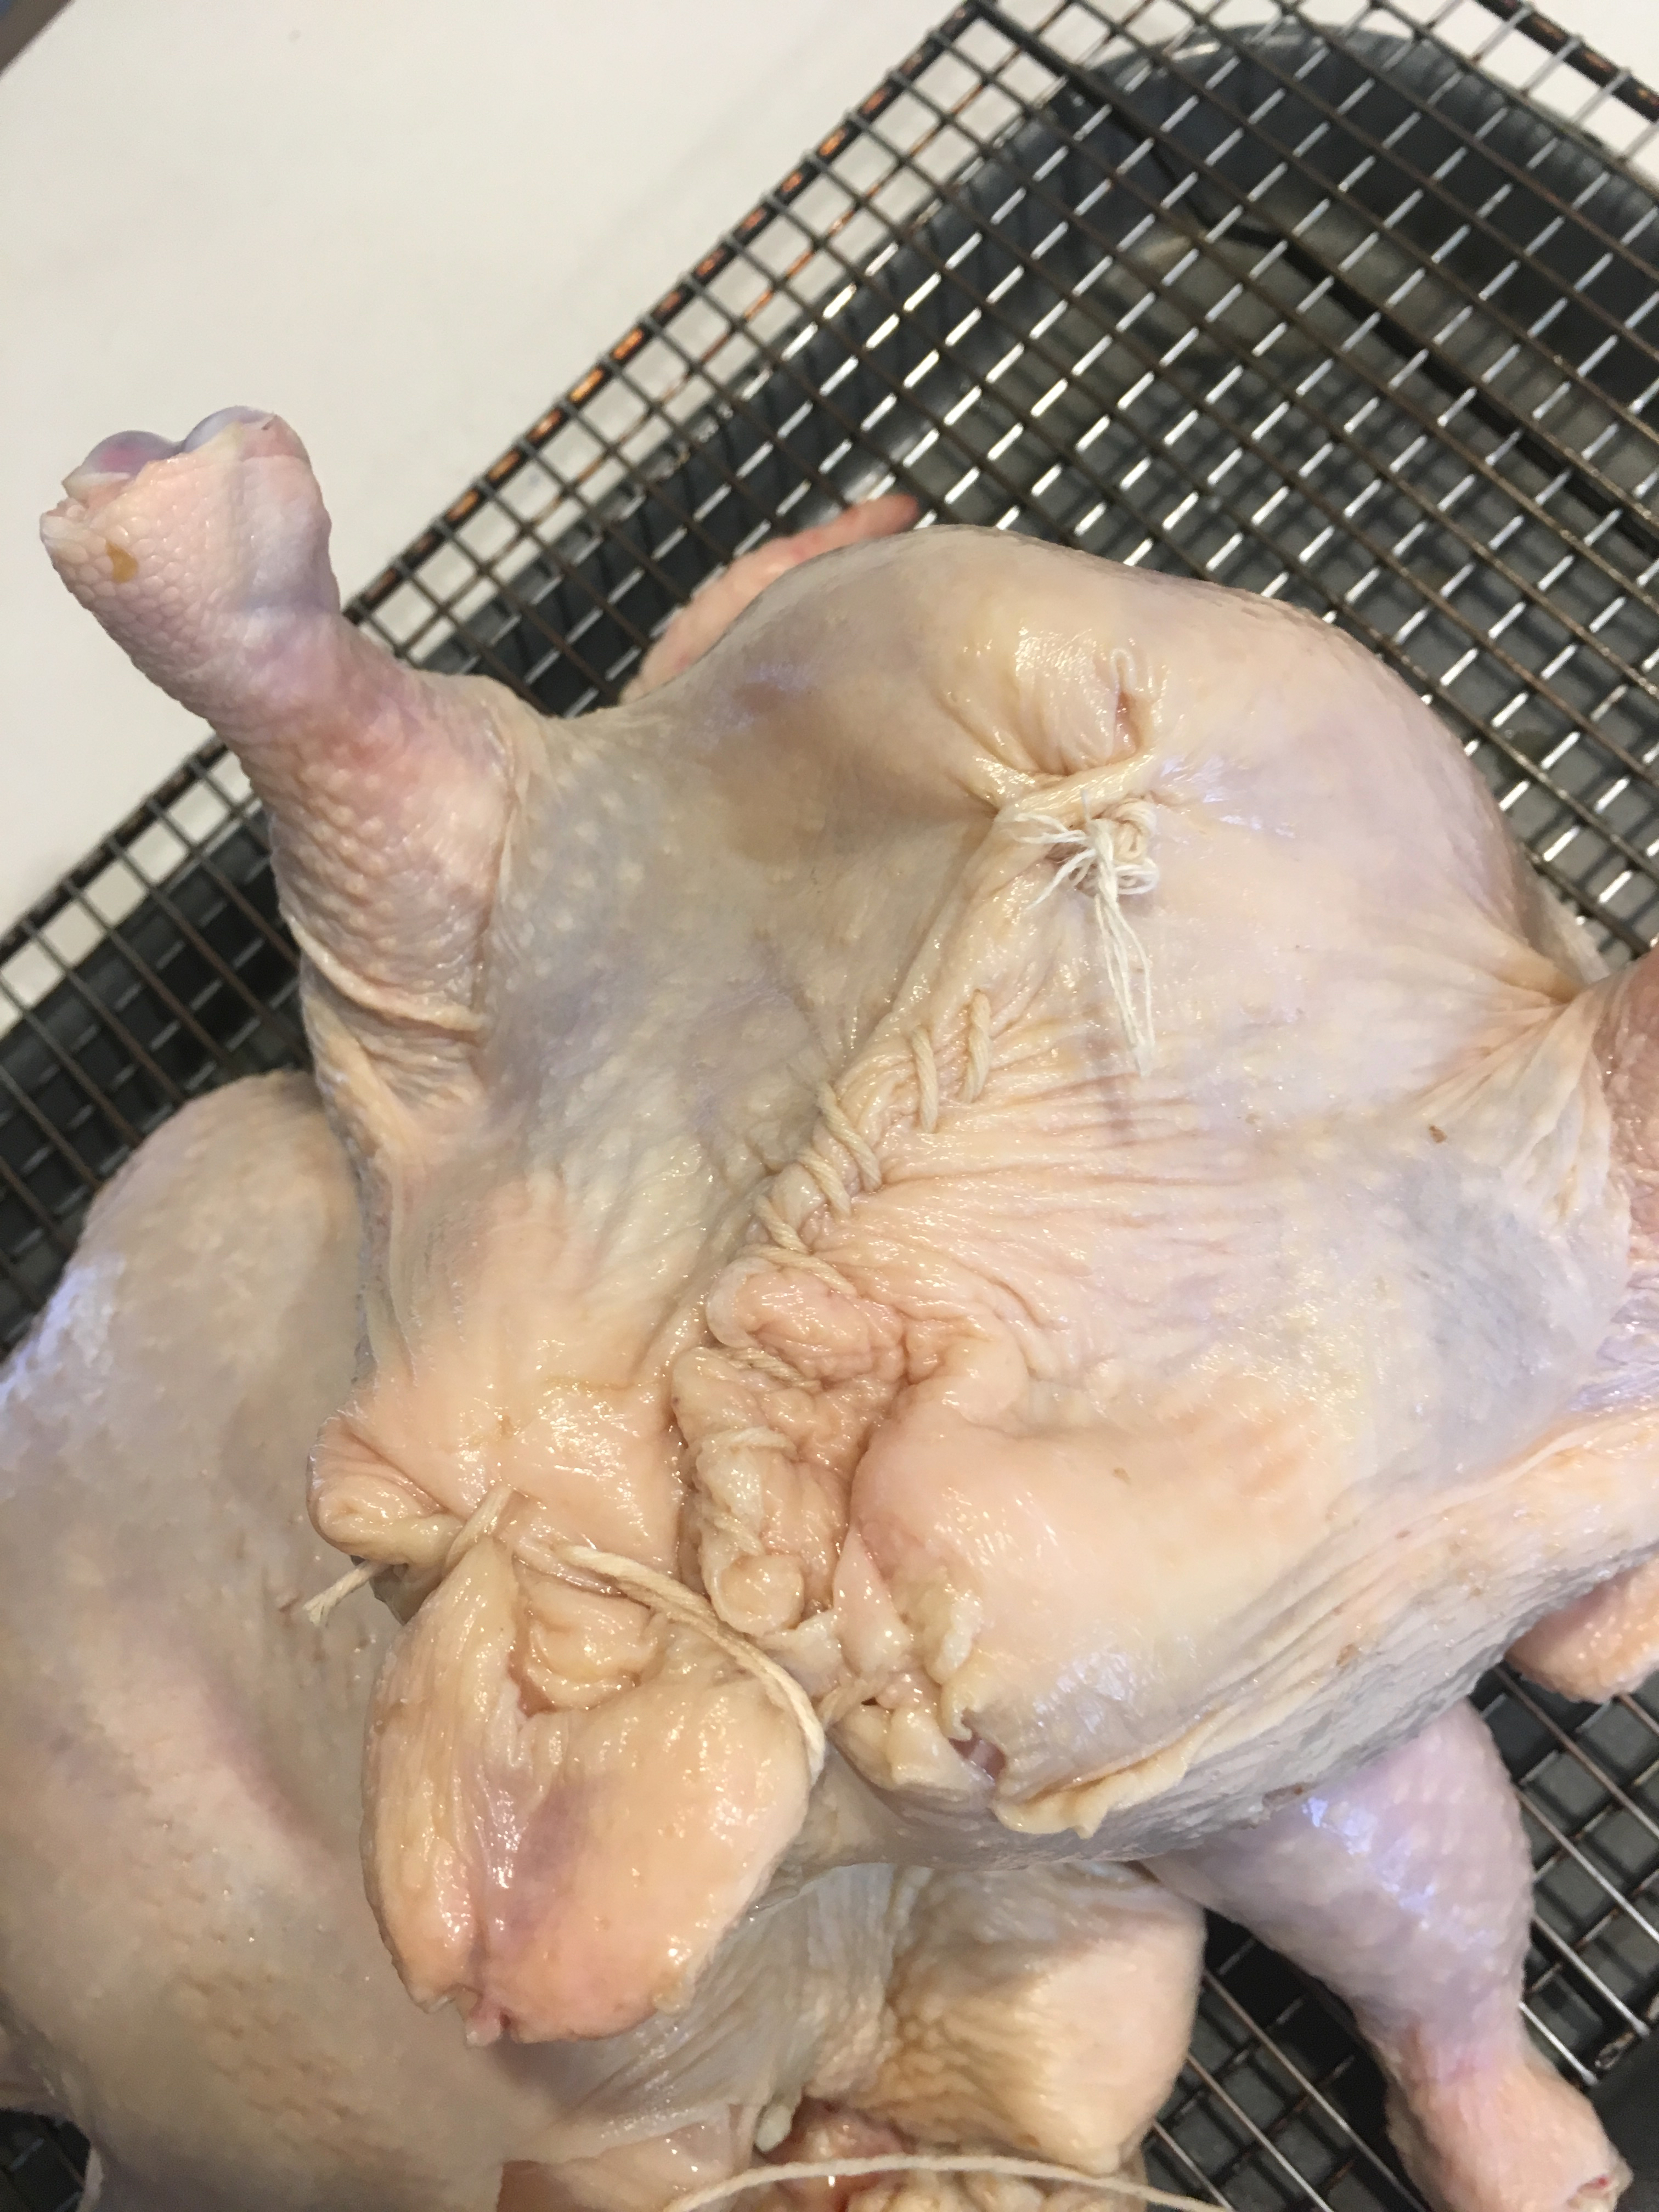
\includegraphics[width=0.25\textwidth]{\imageDir/\fileName/IMG_3217.jpg} &
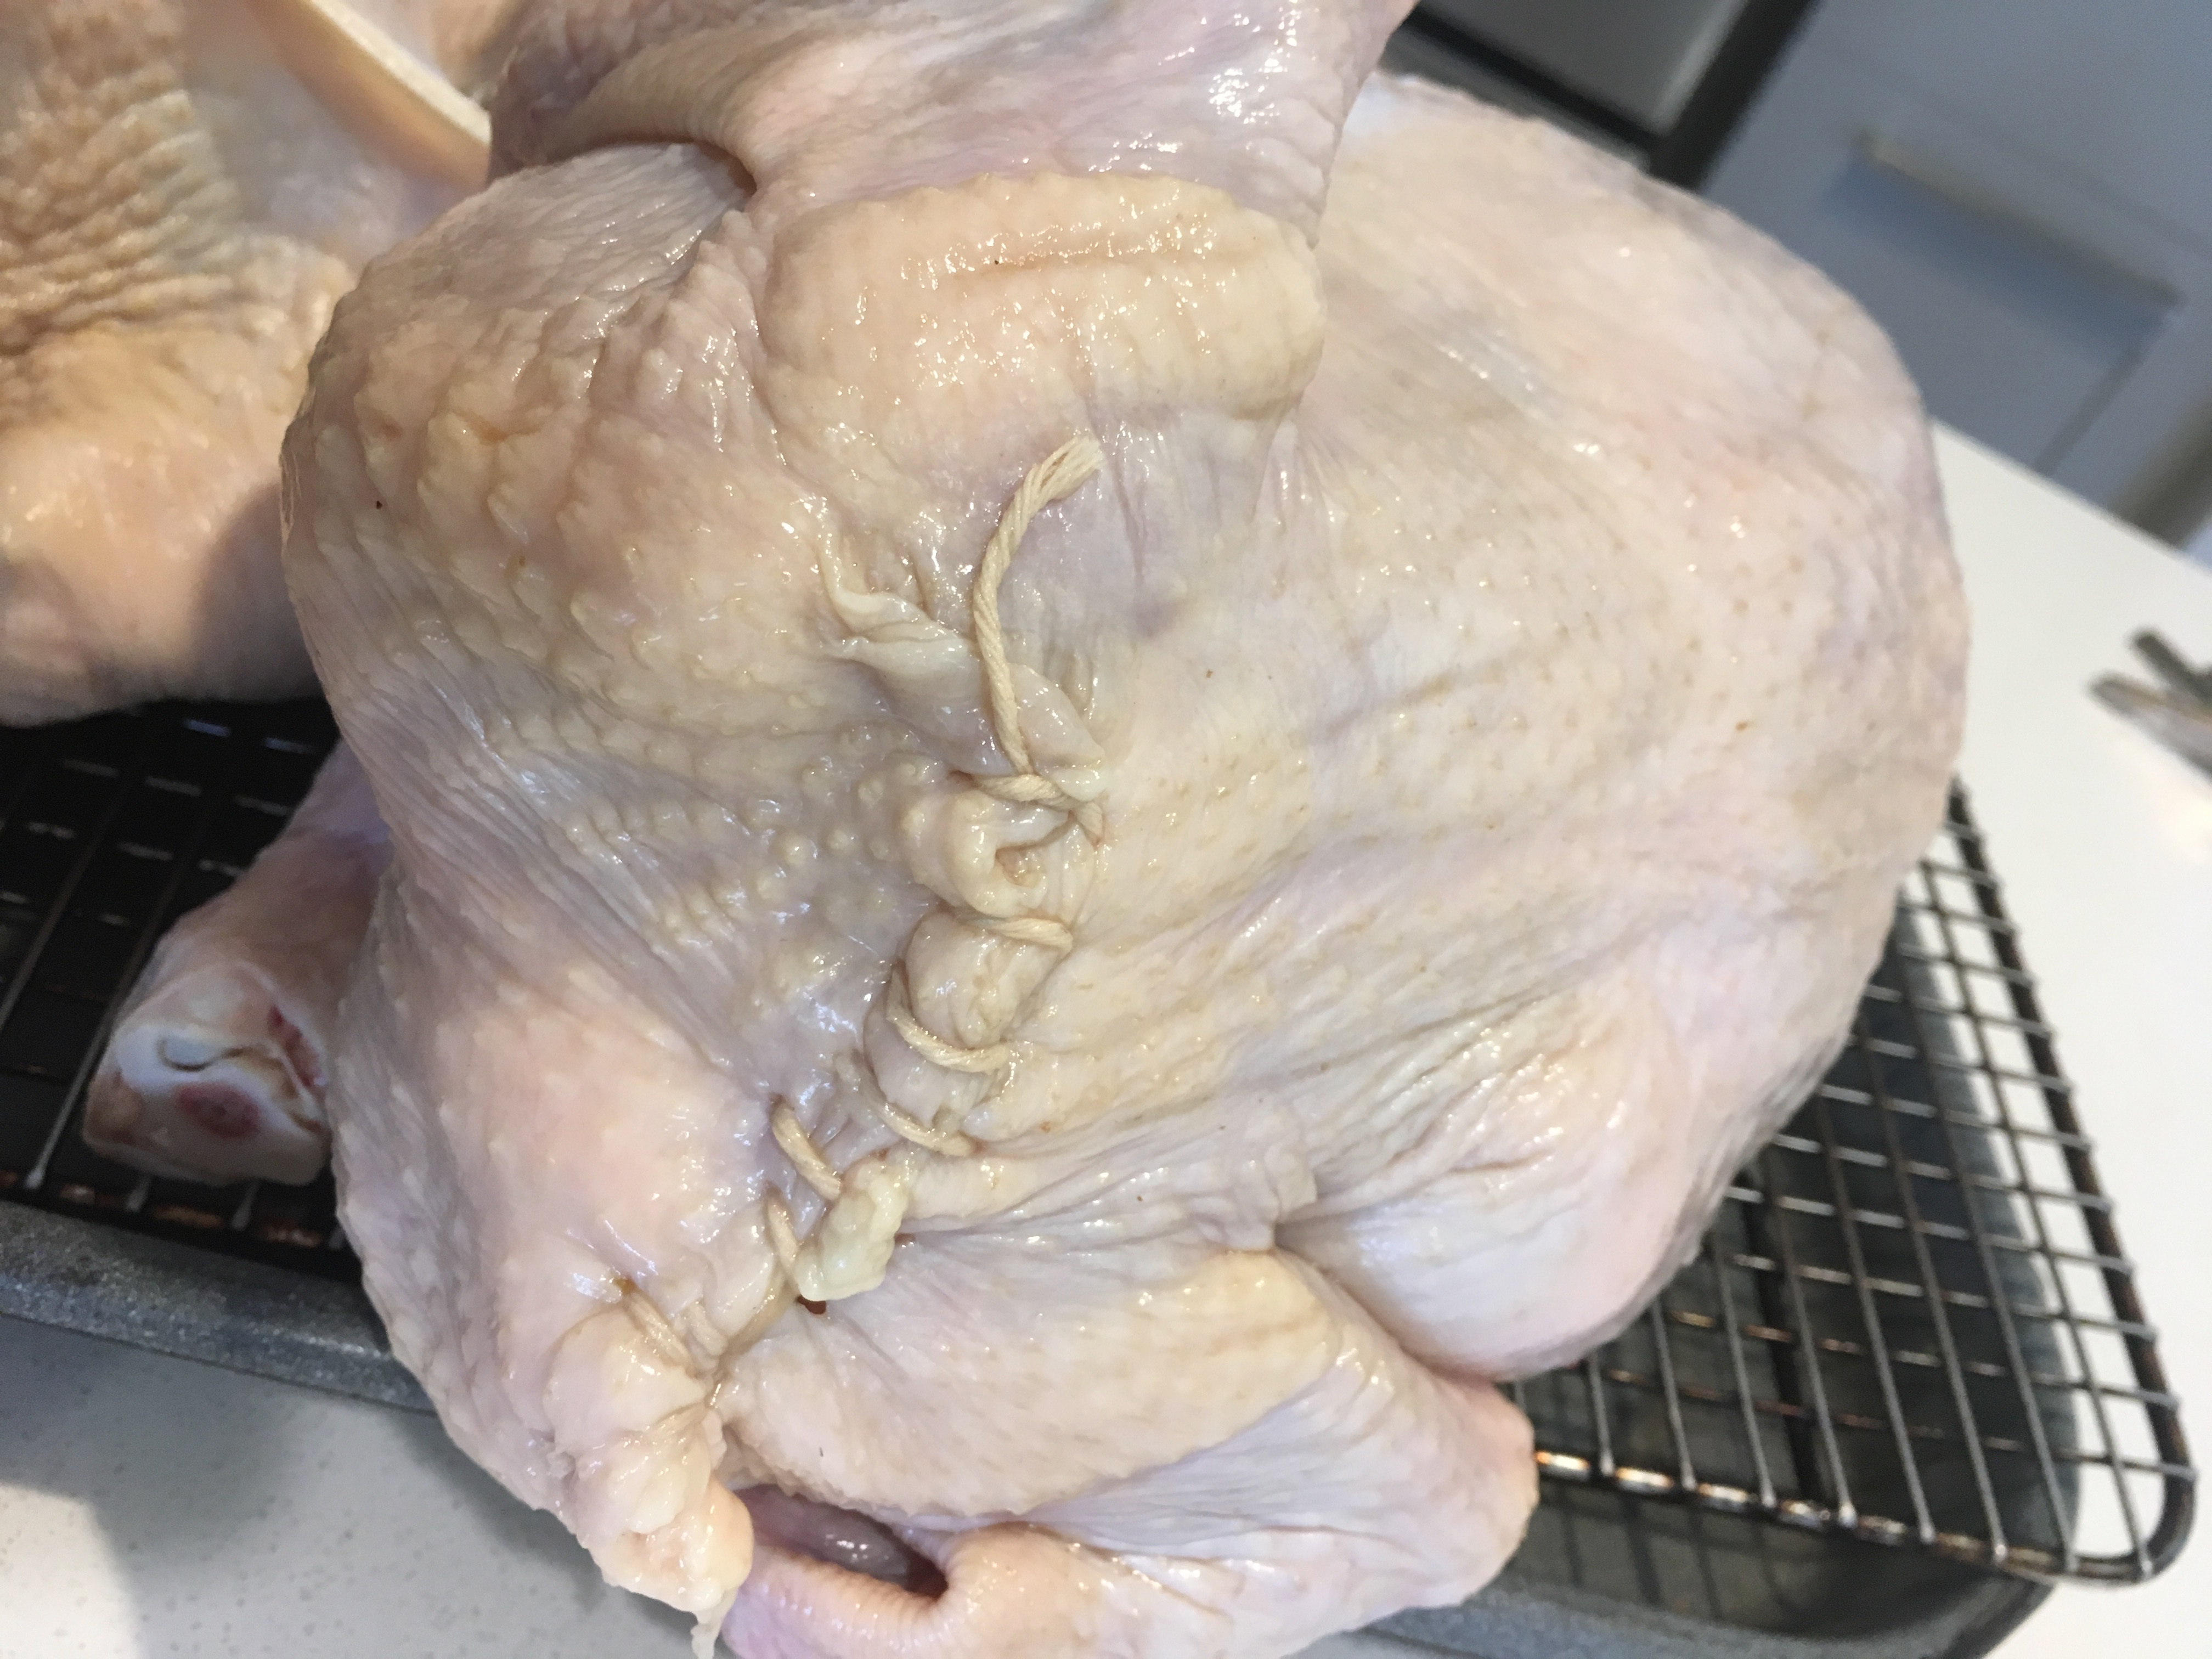
\includegraphics[width=0.25\textwidth]{\imageDir/\fileName/IMG_3218.jpg} &
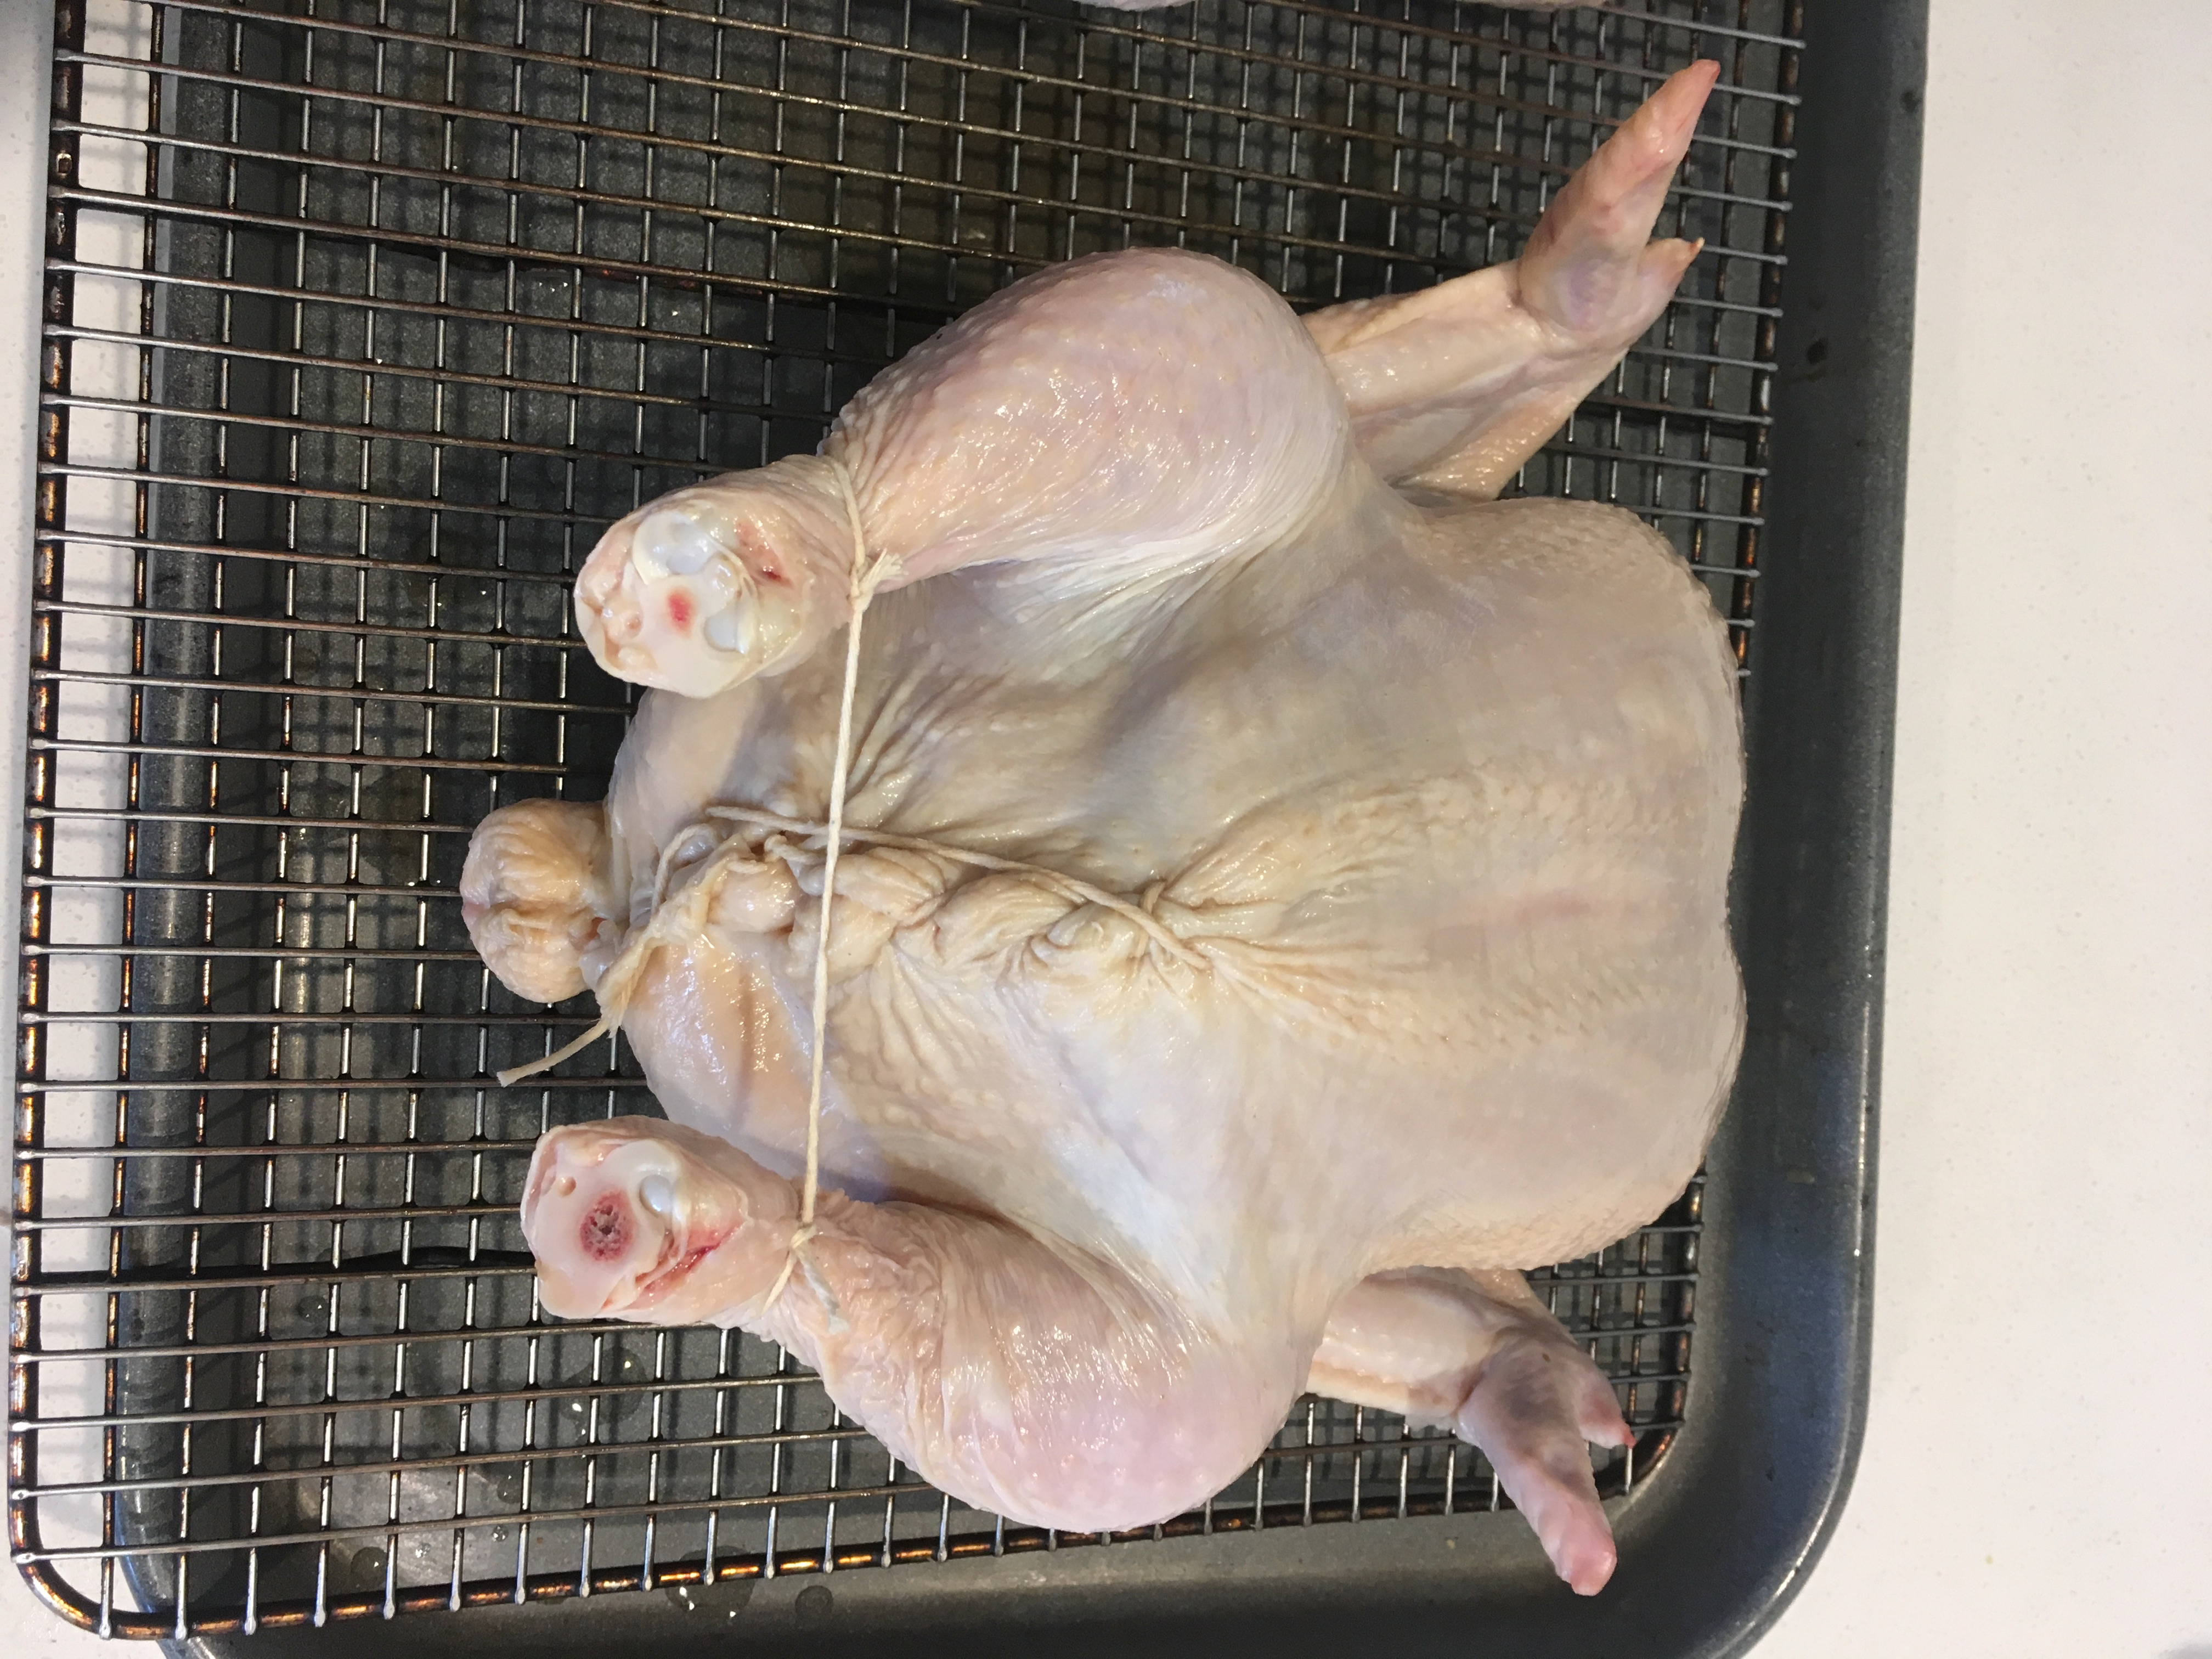
\includegraphics[width=0.25\textwidth]{\imageDir/\fileName/IMG_3219.jpg} \\
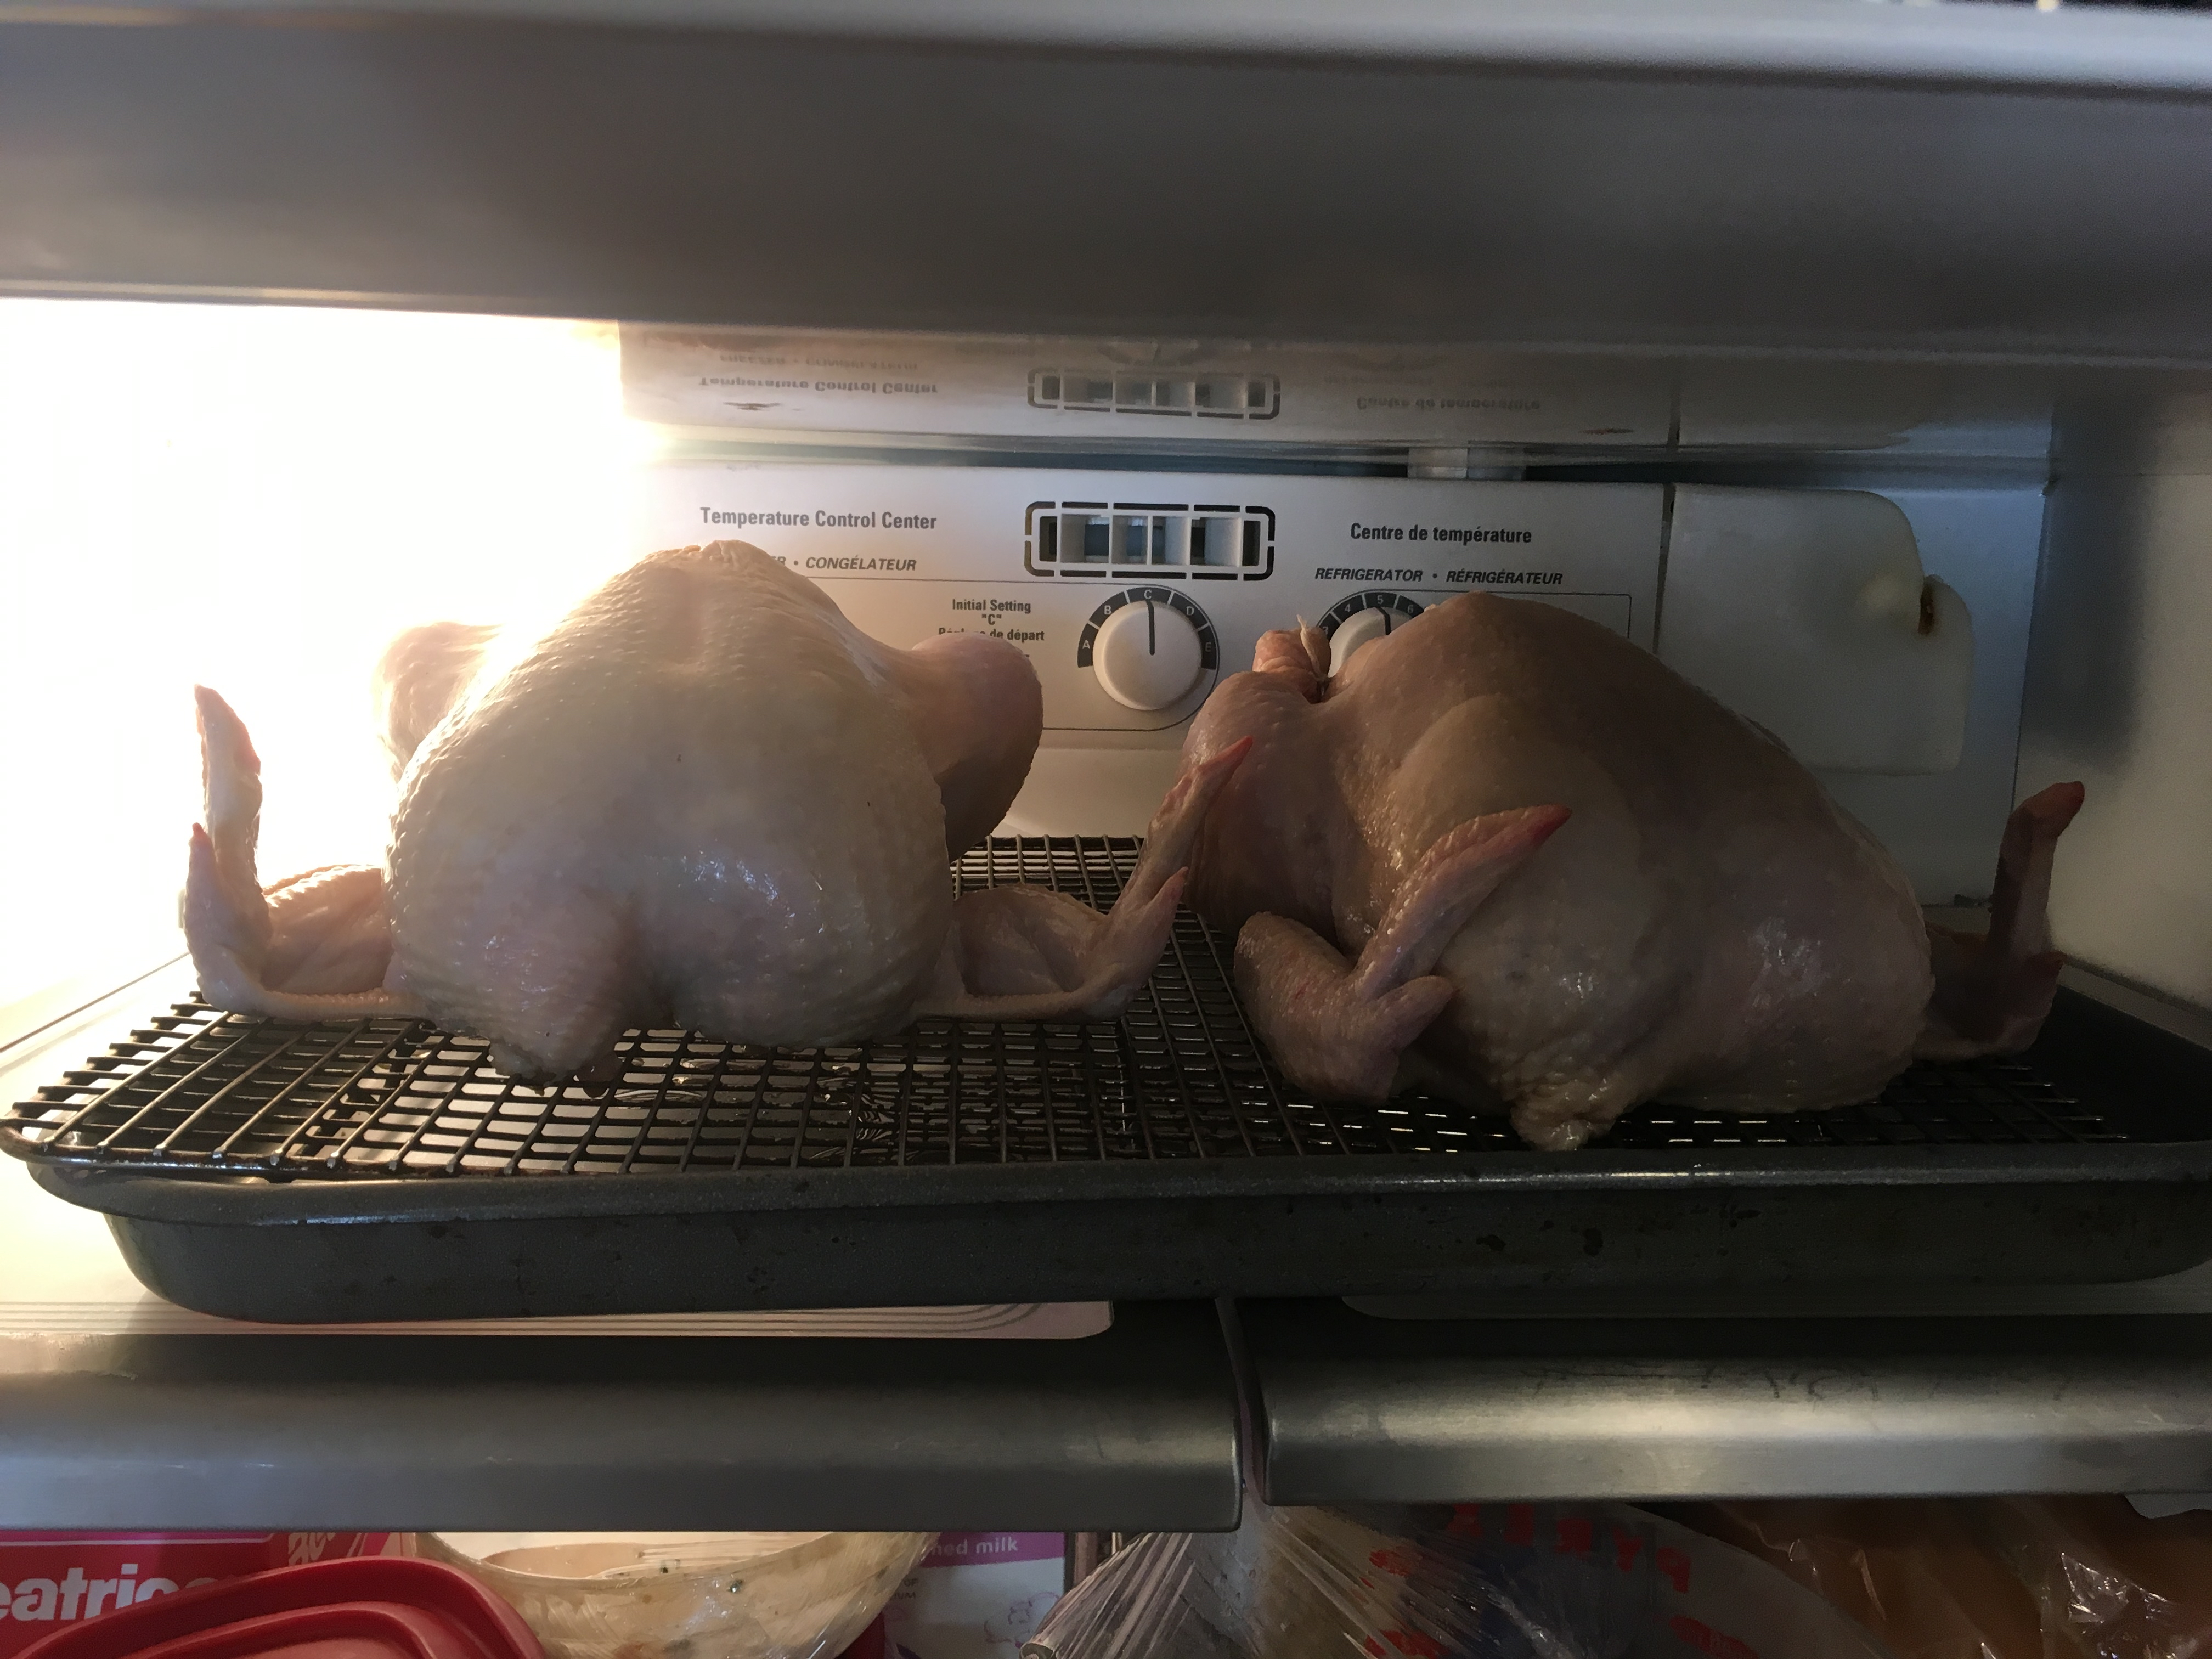
\includegraphics[width=0.25\textwidth]{\imageDir/\fileName/IMG_3220.jpg} &
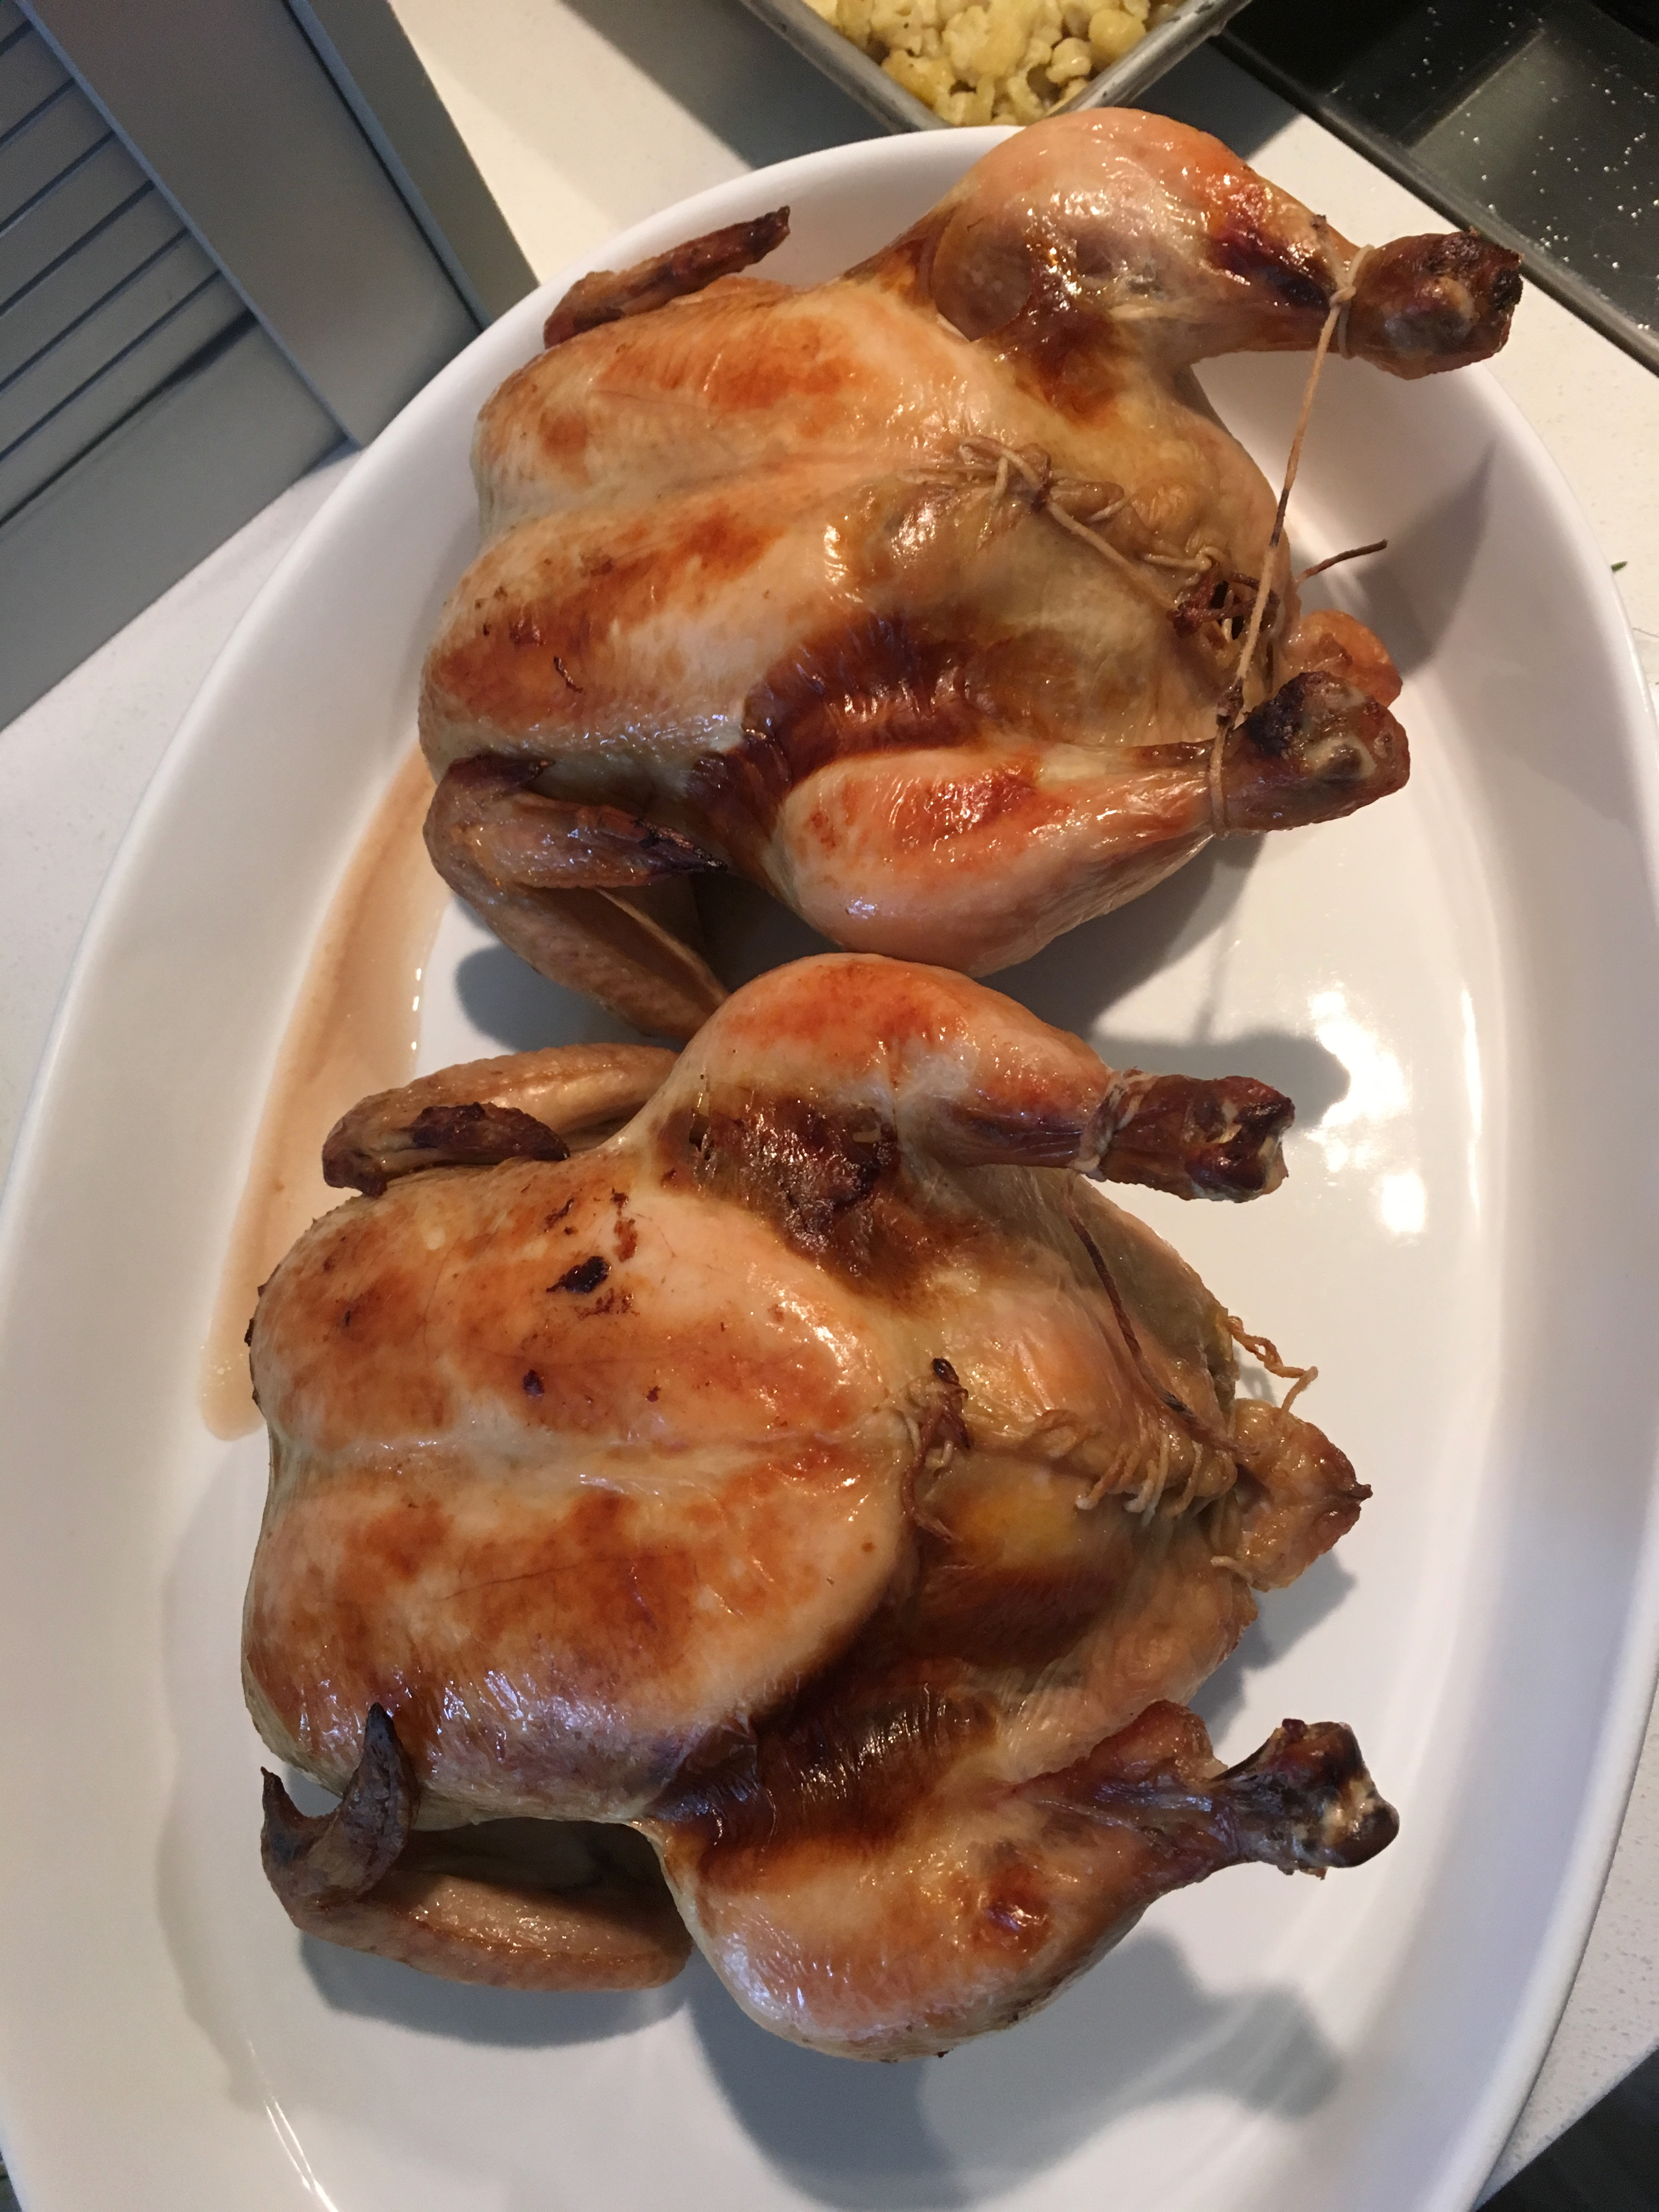
\includegraphics[width=0.25\textwidth]{\imageDir/\fileName/IMG_3228.jpg} \\
\end{tabular}
\end{table}

\end{document}
